\documentclass[twocolumn]{article}

\usepackage[width=17cm,height=22cm]{geometry}
\usepackage[french]{babel}
\usepackage[utf8]{inputenc}
\usepackage{fancyvrb}
\usepackage{authblk}
\usepackage{hyperref}
%% The amssymb package provides various useful mathematical symbols
\usepackage{amssymb}
\usepackage{amsmath}
%% The amsthm package provides extended theorem environments
\usepackage{amsthm}
\usepackage{graphicx}
\usepackage{algorithm}
\usepackage{algorithmic}

\newtheorem{theorem}{Théorème}

\bibliographystyle{alpha}

\title{Expression quadratique de l'apprentissage en ligne d'un bandit contextuel}
\author[1]{Auteur A\thanks{Si vraiment vous voulez mettre votre email
    ou page web...: A.A@univ-x.fr}}
\author[2]{Auteur B}
\affil[1]{Université X, CNRS}
\affil[2]{Université Y, CNRS et INRIA}

\renewcommand\Authands{, et }
\renewcommand\Authand{ et }
\begin{document}
\maketitle

\begin{abstract}
  Ce style est très simple. Vous pouvez ajouter des mots-clef sous le
  résumé. Le nombre de pages est limité à 10. 
\end{abstract}

\medskip

\noindent\textbf{Mots-clef}: Style, \LaTeX, CAP.

\section{Introduction}
\label{sec:lentete}

Les problèmes de bandit contextuels sont au cœur des problématiques de l’apprentissage automatique. Ils abordent en effet, sous une forme très simple, la question de la recherche \emph{active} de l'information de classification. 

Classiquement, l'apprentissage d'un classifieur repose sur une base d'apprentissage constituée par un ensemble de couples $(x_1,y_1),..., (x_n,y_n)$ où le premier terme du couple est un exemple à classer, généralement représenté sous forme vectorielle,  et le deuxième terme une étiquette indiquant la classe de l'exemple fourni.
L'apprentissage consiste alors à déduire une règle générale de classification à partir de ces exemples, pour pouvoir ensuite classer des exemples inconnus.

Il existe cependant de nombreuses situations d'apprentissage dans lesquelles les étiquettes ne sont pas disponibles telles quelles mais sont un peu ``difficiles'' à obtenir. Nous considérons ici le cas du ``bandit contextuel'' qui est une extension des problèmes de bandit manchot au cas de la classification. 

Un problème de bandit simple est constitué d'une part d'un univers,  d'autre part d'un apprenant. L'univers est constitué d'un ensemble fini de machines à sous numérotées de 1 à $K$. Les machines possèdent des bras. Le comportement des machines est stochastique. Lorsqu'on tire un bras, on obtient un gain $g$ variable selon les machines et selon les tirages. Le gain moyen n'est pas le même sur toutes les machines. Certaines machines offrent en moyenne des gains plus élevés que d'autres. Le but de l'apprenant de maximiser son gain total, ce qui revient à découvrir par expérience la ou les machine(s) offrant l'espérance de gain la plus élevée. Pour trouver cette machine optimale, il faut explorer l'univers, c'est à dire essayer toutes les machines, et plusieurs fois si possible afin de collecter une information plus fiable. Le but d'une expérience est ainsi d'une part d'obtenir un bénéfice maximum, mais également de mieux connaître l'univers pour mieux choisir dans le futur les machines les plus favorables. 

Les problèmes de bandit offrent donc un cadre à l'apprentissage actif, au sens où l'information collectée ne dépend pas uniquement des données présentes dans la base, mais également des choix particuliers effectués par l'apprenant. 

Dans ce cadre, on notera un algorithme d'apprentissage selon sa capacité à minimiser le \textit{regret}, qui correspond à l'espérance de la différence entre les gains obtenus à la fin de la partie et le gain qu'on aurait obtenu en appliquant la politique optimale. 
Ainsi, si on considère une séquence de $T$ expériences, le regret se définit comme :
$$R_t = \mathbb{E} \sum_{t=1}^T g_t^* - g_t$$
où $g_t^*$ est le gain obtenu en appliquant la politique optimale et $g_t$ le gain obtenu par l'algorithme d'apprentissage.

Les problèmes de bandit simples se généralisent au cas des bandits dits contextuels \cite{XXX}. Un problème de bandit contextuel est également défini par un univers et un apprenant. L'univers est constitué par des couples (contexte, distribution). Autrement dit, à chaque contexte distinct correspond une distribution de gains distincte sur l'ensemble des $K$ bras. On peut rajouter une hypothèse supplémentaire selon laquelle à des contextes proches correspondent des distributions proches. Le lien avec les problèmes de classification se fait naturellement en considérant des contextes décrits sur des espaces vectoriels, et des catégories décrites par une distribution de gains sur $K$ bras. Dans le cas que nous considérons, à tout contexte $x$ correspond une étiquette unique $y \in \{1,...,K\}$. Autrement dit, en présence de l'exemple $x$, choisir le bras $y$ apporte un gain positif ($g=1$). Pour tout autre choix, le gain est nul ($g=0$). Une expérience consiste ici, en présence du contexte $x$, à choisir une réponse $\tilde{y} \in \{1,...,K\}$. Si $\tilde{y} = y$, le gain vaut 1 sinon il vaut 0. On note $\mathbf{1}_{\tilde{y} = y}$ le gain obtenu dans le cadre de cette expérience. 

Le lien entre ce problème et les problèmes de classification linéaire a été proposé par Kakade \cite{XXX}. Dans le cas de la classification linéaire, des hyperplans séparateurs $w_1, ..., w_K$ définissent les frontières entre les différentes classes dans l'espace des exemplaires.  
Si $x$ est un exemplaire, $\langle w_1, x \rangle > 0$ signifie que $x$ appartient à la classe 1, et $\langle w_1, x \rangle < 0$ qu'il n'appartient pas à la classe 1. Si $x$ est un exemplaire inconnu, on définit généralement la réponse du classifieur comme~:
$$\hat{y} = \arg \max_{k \in\{1,..,K\}}  \langle w_k, x \rangle$$
 
Dans le cadre de l'algorithme ``Banditron'', Kakade propose donc d'apprendre ces hyperplans séparateurs en utilisant un algorithme inspiré du perceptron multiclasse. Il se donne un ensemble de $K$ hyperplans $W_0 = (w^{(1)}_0$, ..., $w^{(K)}_0)$ initialement des vecteurs nuls. A chaque essai, un contexte $x_t$ est lu. Le choix du bras repose sur un tirage aléatoire défini selon~ : $P(\tilde{Y}=k) = (1 - \varepsilon) \mathbf{1}_{k = \hat{y}} + \frac{\varepsilon}{K} $ avec $\varepsilon \in [0,1]$ le paramètre d'exploration. On note $\tilde{y}_t$ le résultat du tirage à l'essai $t$. La mise à jour s'effectue selon~:
$$ W_t = W_{t-1} + \frac{\mathbf{1}_{\tilde{y}_t = y_t} \Phi(x_t,\tilde{y}_t)}{P(\tilde{Y}=\tilde{y}_t)} - \Phi(x_t,\hat{y}_t)$$   
avec $\Phi(x_t,k) = (0, ..., 0,  x_t, 0, .., 0)$ une séquence de vecteurs nuls, excepté à la position $k$ où l'on trouve l'exemplaire $x_t$. Kakade montre que son algorithme converge en espérance vers le classifieur du perceptron, et obtient des garanties sur les bornes d'erreur de son algorithme. 

Toujours dans le cadre des classifieurs linéaires, plusieurs algorithmes d'apprentissage de bandits contextuels ont été proposés dans la littérature. Dans nos expérimentations numériques, nous considérerons également ici l'algorithme ``Confidit'' proposé par Gentile \cite{XXX}, reposant sur le perceptron d'ordre 2 et l'exploration non stochastique basée sur le principe UCB \cite{XXX}, et présentant des profils de convergence plus favorables que le Banditron. 


Dans le cas linéairement séparable, l'apprentissage en ligne d'un perceptron multi-classes peut être significativement accéléré en utilisant les principes de l'optimisation quadratique tels que proposés par Vapnik \cite{XXX}. Dans un article récent, Crammer et al \cite{XXX} proposent une méthode d'apprentissage en ligne supervisée reposant sur l'optimisation locale de la fonction de perte ``hinge loss'' définie dans le cadre multi-classe comme : 
$$
	 l_t =[\mathbf{1}_{\hat{y}_t\neq y_t} + \langle W_{t-1}, \Phi(x_t,y_t)- \Phi(x_t,\hat{y}_t)\rangle]_+ 
$$
où $[.]_+$ retourne l'identité pour les valeurs positives et 0 pour les valeurs négatives. 

La résolution du problème :
$$W_{t} = \arg \min_W \frac{1}{2} \| W - W_{t-1}\|^2 + C \xi^2 \hbox{ s.t. } l_t \leq \xi$$
où $C$ correspond au paramètre d'élasticité, conduit à la mise à jour~:
$$W_{t} =  W_{t-1} + \frac{l_t}{2\|x_t\|^2 + \frac{1}{2C}} (\Phi(x_t,y_t) - \Phi(x_t,\hat{y}_t))$$
Crammer montre que dans le cas linéairement séparable, la somme des pertes au carré est bornée (ce qui est comparable au perceptron). Mais, de manière plus intéressante, il montre également que le regret est  borné dans le cas non séparable.  

\section{Notre approche}

\subsection{Principe}
L'approche adoptée dans le cadre de cet article est une généralisation assez directe des principes d'optimisation quadratique en ligne proposés par Crammer au cas des bandits contextuels. 

L'extension des problèmes d'optimisation en ligne au cas des bandits nécessite de définir une fonction de perte spécifique. 

Soit un classifieur linéaire défini à l'essai $t$ par le jeu de paramètres $W_{t-1}$. Après avoir observé l'exemplaire $x_t$, le choix $\tilde{y}_t$ repose sur un tirage selon la distribution: $$P(\tilde{Y}=k) = (1 - \varepsilon) \mathbf{1}_{k = \hat{y}} + \frac{\varepsilon}{K} $$ avec $\varepsilon \in [0,1]$ le paramètre d'exploration, et $\hat{y}$ la catégorie correspondant au meilleure score des produits salaires entre entre l'exemplaire et les différentes séparatrices.  

Après avoir émis la proposition $\tilde{y}_t$, l'apprenant reçoit un gain $g_t$ égal à 1 si la catégorie proposée est correcte et 0 sinon, soit $g_t = \mathbf{1}_{\tilde{y}_t=y_t}$. 

La perte instantanée est ici définie comme :
$$l_t = [1 + (1 - 2 g_t) \langle W_{t-1}, \Phi(x_t,\tilde{y}_t)\rangle]_+$$
autrement dit~:
\begin{itemize}
	\item[] $l_t = [1 - \langle W_{t-1}, \Phi(x_t,\tilde{y}_t)\rangle]_+$ si $g_t=1$;
	\item[] $l_t = [1 + \langle W_{t-1}, \Phi(x_t,\tilde{y}_t)\rangle]_+$ sinon
\end{itemize}
Dans le premier cas (le choix est correct), la perte décroît avec $\langle W_{t-1}, \Phi(x_t,\tilde{y}_t)\rangle$ jusqu'à 0. Au contraire, dans le second cas (choix incorrect), la perte augmente avec le produit $\langle W_{t-1}, \Phi(x_t,\tilde{y}_t)\rangle$.
Minimiser la perte revient donc à faire croître le produit $\langle W_{t-1}, \Phi(x_t,\tilde{y}_t)\rangle$ dans le premier cas, et à faire décroître le produit $\langle W_{t-1}, \Phi(x_t,\tilde{y}_t)\rangle$  dans le second cas.

La résolution du problème d'optimisation suivant~:
$$W_{t} = \arg \min_W \frac{1}{2} \| W - W_{t-1}\|^2 + C \xi^2 \hbox{ s.t. } l_t \leq \xi$$
où $C$ correspond au paramètre d'élasticité, conduit à la mise à jour~:
$$W_{t} =  W_{t-1} + \frac{l_t}{\|x_t\|^2 + \frac{1}{2C}} (2g_t - 1) \Phi(x_t,\tilde{y}_t)$$

\paragraph{Bandit Passive-Aggressive}
	%\caption{BPA}
	\begin{algorithmic}
		\STATE $\ \ $
		\STATE Parameters:  $\varepsilon\in [0,1]$, $C$.
		\STATE Set $W_0 = 0$ (null vector)
		\FOR {each round $t$ = 1,\dots, $T$}
		\STATE Observe $x_t$.
		\STATE Set $\hat{y}_t = \underset{i = 1,\dots,K}{\text{argmax}}\left\langle W_{t-1} ,\Phi(x_t,i)\right\rangle$
		\FORALL {$i \in [1,...,K]$}
		\STATE $p_{i,t}= (1-\epsilon)\mathbf{1}_{i = \hat{y}_t} + \frac{\epsilon}{K}$
		\ENDFOR
		\STATE Draw $\tilde{y}_t$ randomly from $p_t = \left(p_{1,t},\dots ,p_{K,t}\right)$.
		\STATE Observe $g_t = \mathbf{1}_{(\tilde{y}_t=y_t)}$.
		\STATE Set $l_t = [ 1+(1-2g_t)\left\langle W_{t-1},\Phi(x_t,\tilde{y}_t)\right\rangle]_{+}$ 
		\STATE $W_t = W_{t-1} + (2g_t-1)\frac{l_t}{\parallel\Phi(x_t,\tilde{y}_t)\parallel^2 + \frac{1}{2C}}\cdot\Phi(x_t,\tilde{y}_t)$
		\ENDFOR
	\end{algorithmic}


\subsection{Analyse}
Soit $U$ est un classifieur quelconque de l'espace des classifieurs, on note $l_t^{\ast}$ la perte obtenue par ce classifieur à l'instant $t$. On démontre les deux théorèmes suivants (en négligeant $C$ pour simplifier) :

\begin{theorem}
	\label{theo:BPAT1}
	Let $(x_1,y_1),...,(x_T,y_T)$ be a sequence of separable examples where $x_t \in \mathbb{R}^d$, $y_t\in \{1,...,K\}$ and $\parallel x_t \parallel\leqslant R$ for all t, and $U \in \mathbb{R}^{K\times d}$. Then, the cumulative squared loss of this algorithm is bounded by,
	\begin{equation}
	\sum_{t=1}^{T} l_t^2 \leqslant R^2\cdot \parallel{u}\parallel^2
	\end{equation}
\end{theorem}

\begin{proof}
	Define $\Delta_t$ to be:
	\[\Delta_t = \parallel{W_{t-1}-U}\parallel^2-\parallel{W_t-U}\parallel^2\]
	By summing $\Delta_t$ over all $t$ from 1 to $T$,  $\sum_t \Delta_t$ is shown to be a telescopic sum which collapses to
	\begin{align}
    \sum_{t=1}^{T}\Delta_t &= \sum_{t=1}^{T} \left( \parallel{W_{t-1} - U}\parallel^2-\parallel{W_t - U}\parallel^2 \right)\nonumber\\ 
    &= \parallel{W_0 - U}\parallel^2-\parallel{W_t-U}\parallel^2\nonumber
	\end{align}	
	By the initiation of $W_0 = \vec{0}$, 
	\begin{equation}
	\label{equa:delta}
	\sum_{t=1}^{T}\Delta_t = \parallel{U}\parallel^2 - \parallel{W_t-U}\parallel^2 \leqslant \parallel{U}\parallel^2 
	\end{equation}
	
	Using the definition of update : %in Eq.\ref{eq:,
	\begin{align}
	\Delta_t =& -2\left\langle (W_{t-1} - U), (2g_t-1)\frac{l_t}{\parallel{x_t}\parallel^2}\Phi(x_t,\tilde{y}_t)\right\rangle \nonumber\\
	&- \left\| \frac{l_t}{\parallel{x_t}\parallel^2}\Phi(x_t,\tilde{y}_t)\right\|^2
	\nonumber
	\end{align}
	%With  $l_t = [1+(1-2\1_{(\tilde{y}_t = y_t)})\cdot\langle w_t,\Phi(x_t,\tilde{y}_t)\rangle]_+$  and  $l_t^{\ast} = [1+(1-2\1_{(\tilde{y}_t = y_t)})\cdot\langle u,\Phi(x_t,\tilde{y}_t)\rangle]_+$ ,
	So, 
	\begin{align}
	\Delta_t &= 2\frac{l_t^2 - l_t l_t^{\ast}}{\parallel{x_t}\parallel^2}-\left( \frac{l_t}{\parallel{x_t}\parallel^2}\parallel{\Phi(x_t,\tilde{y}_t)}\parallel \right)^2\nonumber\\
	&= \frac{l_t^2-2l_t l_t^{\ast}}{\parallel x_t\parallel^2}\nonumber
	\end{align}
	If all examples are separable, $\exists U$ such that $\forall t \in [1,...,T]$ , $l_t^{\ast} = 0$ ,
	%, following the Eq.~\ref{sumDelta},
	
	\[\Rightarrow \parallel{U}\parallel^2 \geqslant \sum_{t=1}^{T}\Delta_t \geqslant \sum_{t=1}^{T}  \frac{l_t^2}{\parallel{x_t}\parallel^2}\]
	\[\Rightarrow \sum_{t=1}^{T} l_t^2 \leqslant\parallel{U}\parallel^2 \cdot \parallel{\Phi(x_t,\tilde{y}_t)}\parallel^2\]
	\[\sum_{t=1}^{T} l_t^2 \leqslant R^2 \cdot \parallel{U}\parallel^2\]
\end{proof}
\begin{theorem}
	\label{theo:BPAT2}
	Let $(x_1,y_1),...,(x_T,y_T) $ be a sequence of non-separable examples where  $x_t\in \mathbb{R}^d$, $y_t \in \{1,...,K\}$ and $\parallel{x_t}\parallel \leqslant R$ for all t. Then for any  $U \in \mathbb{R}^{K\times d}$, the cumulative squared loss of this algorithm is bounded by:
	\[\sum_{t=1}^{T}l_t^2 \leqslant \left(R\parallel{U}\parallel+2 \sqrt{\sum_{t=1}^{T}(l_t^{\ast})^2}\right)^2 \]
\end{theorem}
\begin{proof}
	By the proof of Theorem \ref{theo:BPAT1}, 
	\[\sum_{t=1}^{T}l_t^2 \leqslant R^2\cdot \parallel{u}\parallel^2 + 2\sum_{t=1}^{T}l_t l_t^{\ast}\]
	To upper bound the right side of the above inequality, we denote $A_t = \sqrt{\sum_{t=1}^{T}l_t^2}$ and $B_t = \sqrt{\sum_{t=1}^{T}(l_t^{\ast})^2}$, 
	\begin{align}
	2(A_tB_t)^2-2(\sum_{t=1}^{T}l_tl_t^{\ast})^2 =& \sum_{i=1}^{T}\sum_{j=1}^{T}l_i^2(l_j^{\ast})^2+\sum_{i=1}^{T}\sum_{j=1}^{T}l_j^2(l_i^{\ast})^2 \nonumber\\
	&- 2\sum_{i=1}^{T}\sum_{j=1}^{T}l_il_jl_i^{\ast}l_j^{\ast}\nonumber\\
	=& \sum_{i=1}^{T}\sum_{j=1}^{T}(l_il_j^{\ast}-l_jl_i^{\ast})^2 \geqslant 0 \nonumber
	\end{align}
	
	\begin{align}
	\sum_{t=1}^{T}l_t^2 \leqslant R^2 \cdot \parallel{U}\parallel^2+2\sum_{t=1}^{T}l_tl_t^{\ast}\leqslant R^2 \cdot \parallel{u}\parallel^2+2A_tB_t
	\end{align}
	%\[L_t^2 -2R^2 L_tU_t+U_t^2\leqslant R^2\parallel{u}\parallel^2+U_t^2\]
	\[A_t \leqslant B_t+\sqrt{R^2\parallel{U}\parallel^2+B_t^2}\]
	Using the fact that $\sqrt{a+b}\leqslant \sqrt{a}+\sqrt{b}$,
	\[A_t \leqslant R\parallel{U}\parallel+2 B_t\]
	\[\sum_{t=1}^{T}l_t^2 \leqslant \left(R\parallel{U}\parallel+2 \sqrt{\sum_{t=1}^{T}(l_t^{\ast})^2}\right)^2 \]
\end{proof}

%Pour les affiliations, vous pouvez utiliser
%\href{http://ctan.org/pkg/authblk}{le paquet \texttt{authblk}}.

\subsection{Extensions}
Le plongement des données d'entrée dans des espaces de Hilbert à noyaux reproduisants (RKHS) permet d'étendre notre approche aux jeux de données non linéairement séparables. 

Soit $\mathcal{H}$ un espace de Hilbert à noyaux reproduisants dont le produit scalaire est défini à l'aide de la fonction noyau $\mathcal{K}$. On note $\mathcal{K}(x,.)$ la projection de l'exemplaire $x$ dans $\mathcal{H}$, avec $\forall f \in \mathcal{H}, \langle f,\mathcal{K}(x,.)\rangle_\mathcal{H} = f(x) $.
 

Le classifieur est dans ce cadre défini comme un ensemble de fonctions : $\mathcal{F} = \{f^{(1)}, ..., f^{(K)}\}$ avec :
$$\hat{y} = \arg \max_k f^{(k)}(x)$$

Soit $\mathcal{F}_0=\{0, ..., 0\}$ le classifieur initial. A chaque essai, est mis à jour selon la règle définie précédemment, soit à l'instant $t$~:
$$\mathcal{F}_t = \{f^{(1)}_t, ..., f^{(K)}_t\}$$
$$\forall k, f^{(k)}_t = \sum_{t^\prime = 1} ^t  \frac {\mathbf{1}_{k=\tilde{y}_{t^\prime}}l_{t^\prime}}{\mathcal{K}(x_{t^\prime},x_{t^\prime})} (2g_{t^\prime} - 1)\mathcal{K}(x_{t^\prime},.)$$
$$ l_t = [1 + (1-2g_t) f_{t-1}^{(\tilde{y}_t)}(x_t)]_+$$
%Et évidemment, vous ajoutez ensuite les paquets que vous voulez
%utiliser, les macros les définitions de théorèmes etc... Nous
%recommandons le paquet \texttt{hyperref} puisque les documents
%\texttt{PDF} seront en ligne si vous avez donné votre accord.

\section{Experiments}

\subsection{High-dimensional datassets}
\label{subsec:BPAE}
Here, we evaluate the algorithms over two synthetic and three real world data sets. Their characteristics are summarized in Table~\ref{table:mce}.

\begin{table}[h]
	\caption{Summary of the three high-dimensional datasets, including the numbers of instances, features, labels and whether the number of examples in each class are balanced.}
	\label{table:mce}
	\begin{center}
		\begin{tabular}{l l l l l}
			{\bf Dataset}  & {\bf Instances} & {\bf Features} & {\bf Labels}& {\bf Balanced}\\
			\hline
			SynSep & $10^5$ 	& 400 	& 9 & Y\\
			
			SynNonSep & $10^5$ & 400 	& 9 & Y\\
			
			RCV1-v2  & $10^5$ 	& 47236 	& 53 & N\\
			
			%Letter 	&$2*10^4$	&16	&26	&N\\
			
			%Pen-Based &$1.32*10^4$	&16	&10	&N\\
		\end{tabular}
	\end{center}
\end{table}

\textbf{Data sets}:
The first data set, denoted by SynSep,  is a 9-class, 400-dimensional synthetic data set of size $10^5$. More details about the method to generate this data set can be found in \cite{kakade2008efficient}. The SynSep  idea is to have a simple simulation of generating a text document. The coordinates represent different words in a small vocabulary of size $400$. We ensure that SynSep is linearly separable. 

The second data set, denoted by SynNonSep, is constructed  the same way as  SynSep except that a 5\% label noise is introduced, which makes the data set non-separable. 

The third data set is collected from the Reuters RCV1-v2 collection\cite{David04RCV}. The original data set is composed by multi-label instances. So we make some preprocessing likes \cite{RB08a}. First, its label hierarchy is reorganized by mapping the data set to the second level of RCV1 topic hierarchy. The documents that have labels of the third or forth level only are mapped to their parent category of the second level; Second, all multi-labelled instances have been removed. This RCV1-v2 is a 53-class,  47236-dimensional real data set of size $10^5$. 

%The fourth and fifth data sets are collected from \cite{letter26SC,number10SC}. The fourth data set is to identify each of a large number of black-and-white rectangular pixel displays as one of the 26 capital letters in the English alphabet. The character images were based on 20 different fonts and each letter within these 20 fonts was randomly distorted to produce a file of 20000 unique stimuli. Each stimuli was converted into 16 primitive numerical attributes (statistical moments and edge counts). It forms a 26-class, 16-dimensional real data set of size $20000$. The fifth data set is a digit data base made by collecting 250 samples from 44 writers, using only (x,y) coordinate information represented as constant length feature vectors, which were resampled to 8 points per digit (therefore the data set contains 8 points $\times$ 2 coordinates = 16 features). This one is a 10-class, 16-dimensional real data set of size $10992$.

\textbf{Results}
Figures \ref{pic:BPASS} and~\ref{pic:BPASNS} show the experimental results on two synthetic data sets. For SynSep, a separable linear data set, all algorithms except Banditron obtain a good performance; with the non-separable SynNonSep data, Confidit and BPA outperform the other algorithms, even the supervised algorithms.  To different datasets, the parameters of different algorithms refer to Table~\ref{table:bpa}.
\begin{table}[h]
	\caption{The summary of algorithm parameters for different datasets. P. denotes Perceptron, PA is Passive-Aggressive online algorithm, B. is Banditron, C. is Confidit and BPA.}
	\label{table:bpa}
	\begin{center}
		\begin{tabular}{lllllll}
			{\bf Dataset}  & {\bf P.} & {\bf PA } & {\bf B.}& {\bf C.} & {\bf BPA}\\
			\hline
			SynSep & null & $C=0$ & $\varepsilon = 0.014$ &$\eta = 10^3$ & $\varepsilon = 0.4,C = 0$\\
			
			SynNonSep & null & $C=10^{-2}$ & $\varepsilon =0.65$ & $\eta = 10^3$& $\varepsilon = 0.8,C = 10^{-2}$\\
			
			Reuters & null & $C=10^{-2}$ & $\varepsilon =0.4$ & $\eta = 10^2$ & $\varepsilon = 0.2,C = 10^{-2}$\\
			
			%LR(26 letters) & null &  $C=0.1$ & $\varepsilon = 0.2$& $\eta=10^2$ & $\varepsilon = 0.8,C= 1$ \\
			
			%LR(10 numbers) & null & $C=0.1$ & $\varepsilon= 0.4$& $\eta = 10$ & $\varepsilon = 0.6,C=1$\\
			
		\end{tabular}
	\end{center}
\end{table}

%\textcolor{red}{OK-- Il manque les valeurs des paramètres pour les différents algorithmes (faire un tableau comme dans la partie précédente).}

Figure~\ref{pic:BPARCV} %, ~\ref{pic:BPALR10} and~\ref{pic:BPALR26} 
presents the result on the real dataset. With this dataset, the supervised algorithms, despite their competitive advantage with respect to the ones with bandit feedback, do not significantly depart from BPA and Confidit, with classification results that clearly outperform Banditron. While having a lower computational complexity, BPA approach is even found to outperform Confidit in the most challenging situation, i.e. the high-dimensional case with a large number of classes (RCV1-v2 data set).

The $\epsilon$ parameter represents the exploration rate in Banditron and BPA algorithms. We compare on Figure 3 the average error rates obtained on the two algorithms for different values of $\epsilon$ on the different data sets. In contrast with Banditron, BPA shows that $\epsilon$ has a very little influence on the final error rate, indicating a capability to deal with small exploration rates.


\begin{figure}[h!]
	
	\centerline{
		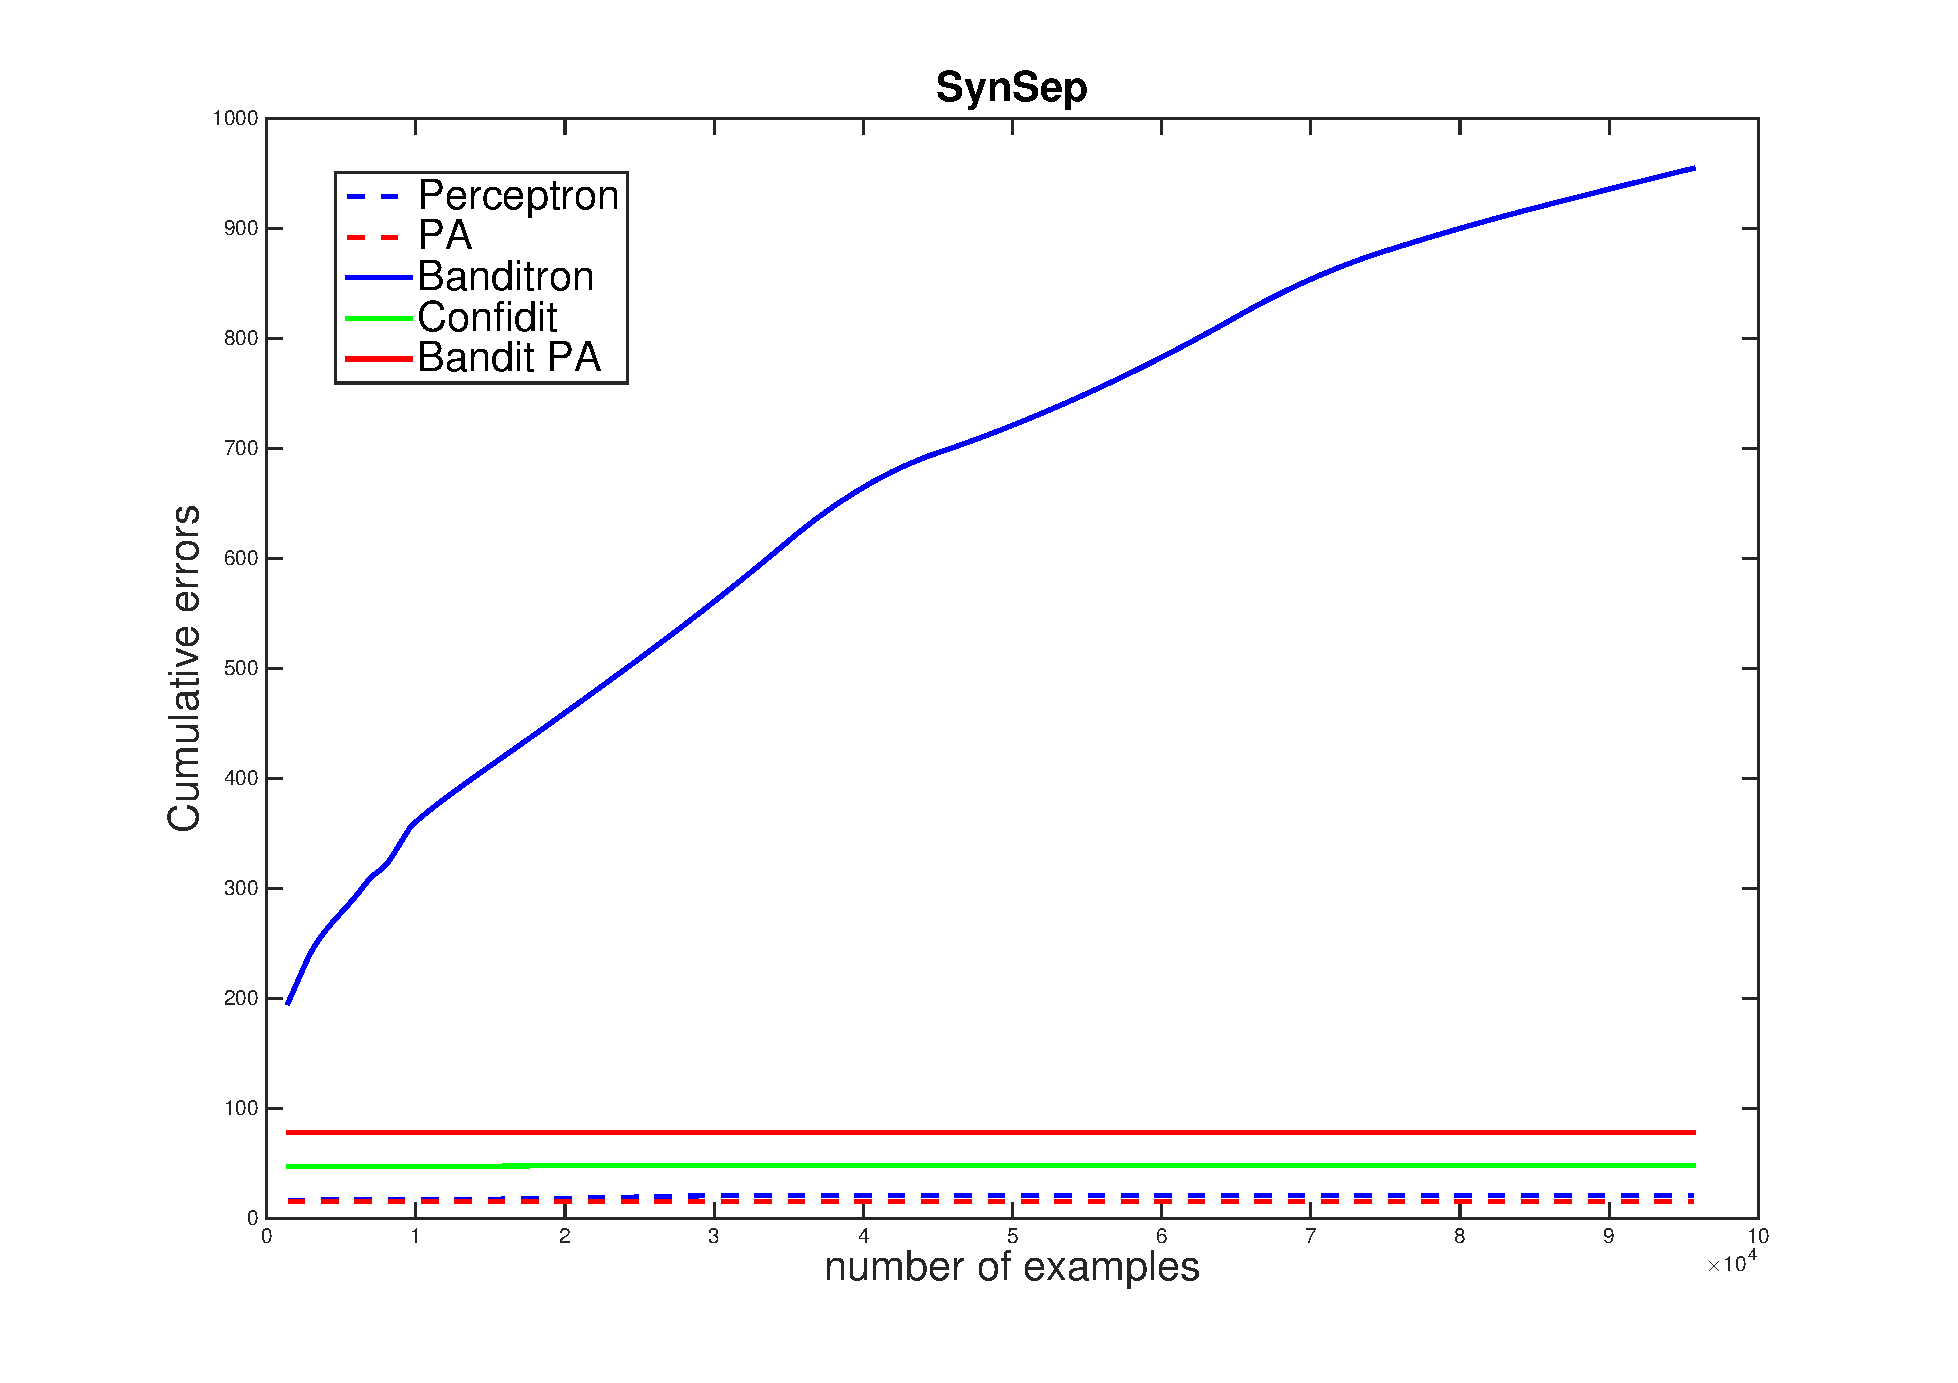
\includegraphics[width=\linewidth]{figs/SynSep.eps}
	}
	\caption{Cumulative Errors on the synthetic data set of  SynSep.}
	\label{pic:BPASS}
\end{figure}
\begin{figure}[h!]
	
	\centerline{
		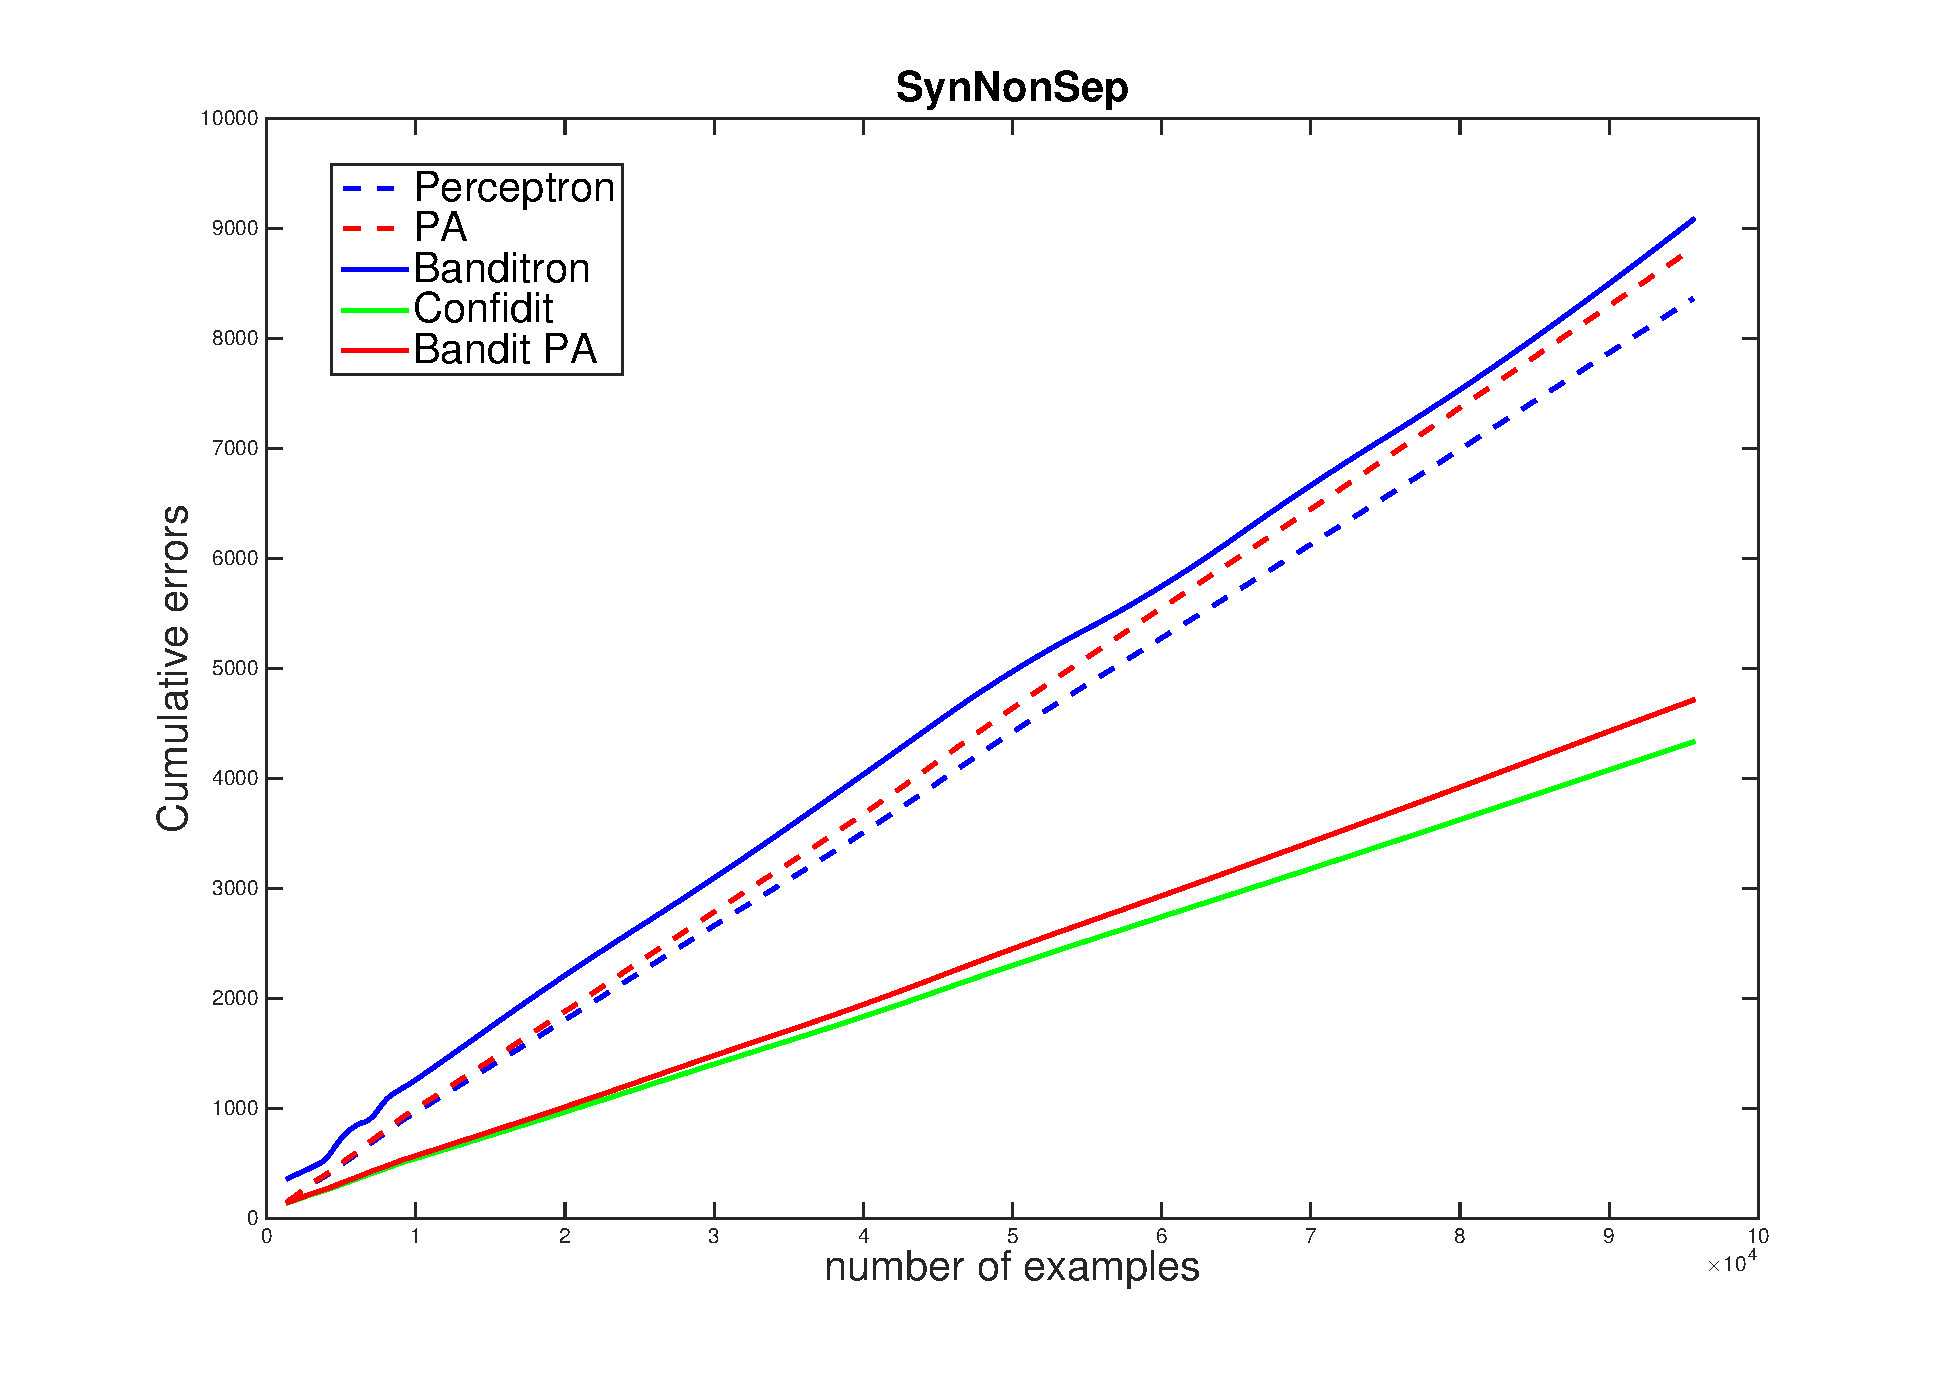
\includegraphics[width=\linewidth]{figs/SynNonSep.eps}
	}
	\caption{Cumulative Errors on the synthetic data set of SynNonSep.}
	\label{pic:BPASNS}
\end{figure}
\begin{figure}[h!]
	\centerline{
		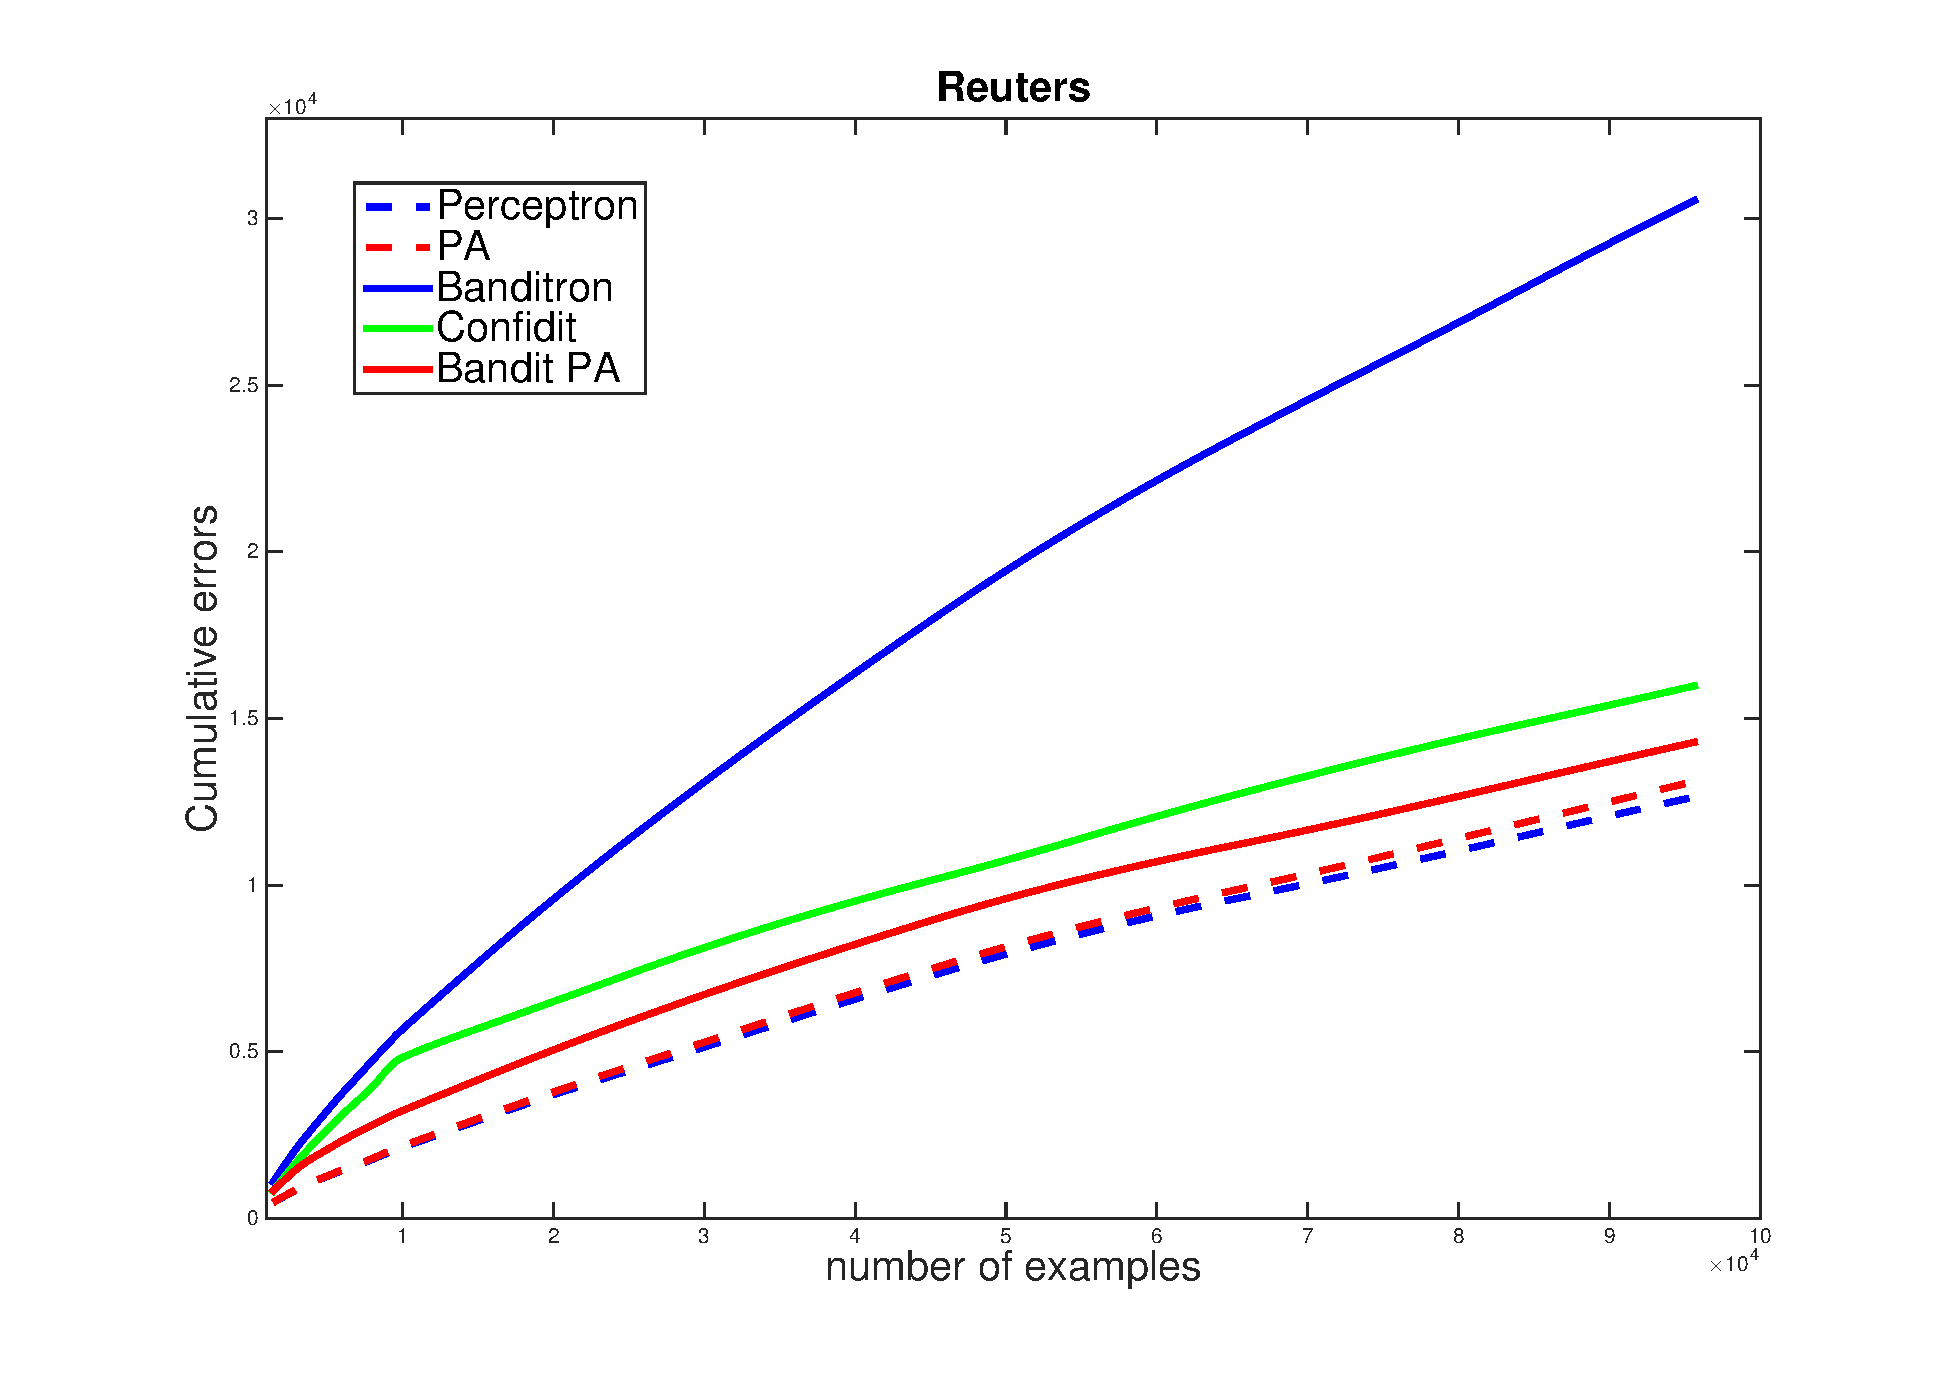
\includegraphics[width=\linewidth]{figs/RCV1_v2_53class.eps}}
	\caption{Cumulative Errors  on the real data set of RCV1-v2 (53 classes).}
	\label{pic:BPARCV}
\end{figure}

\begin{figure}[h!]
	\centerline{
		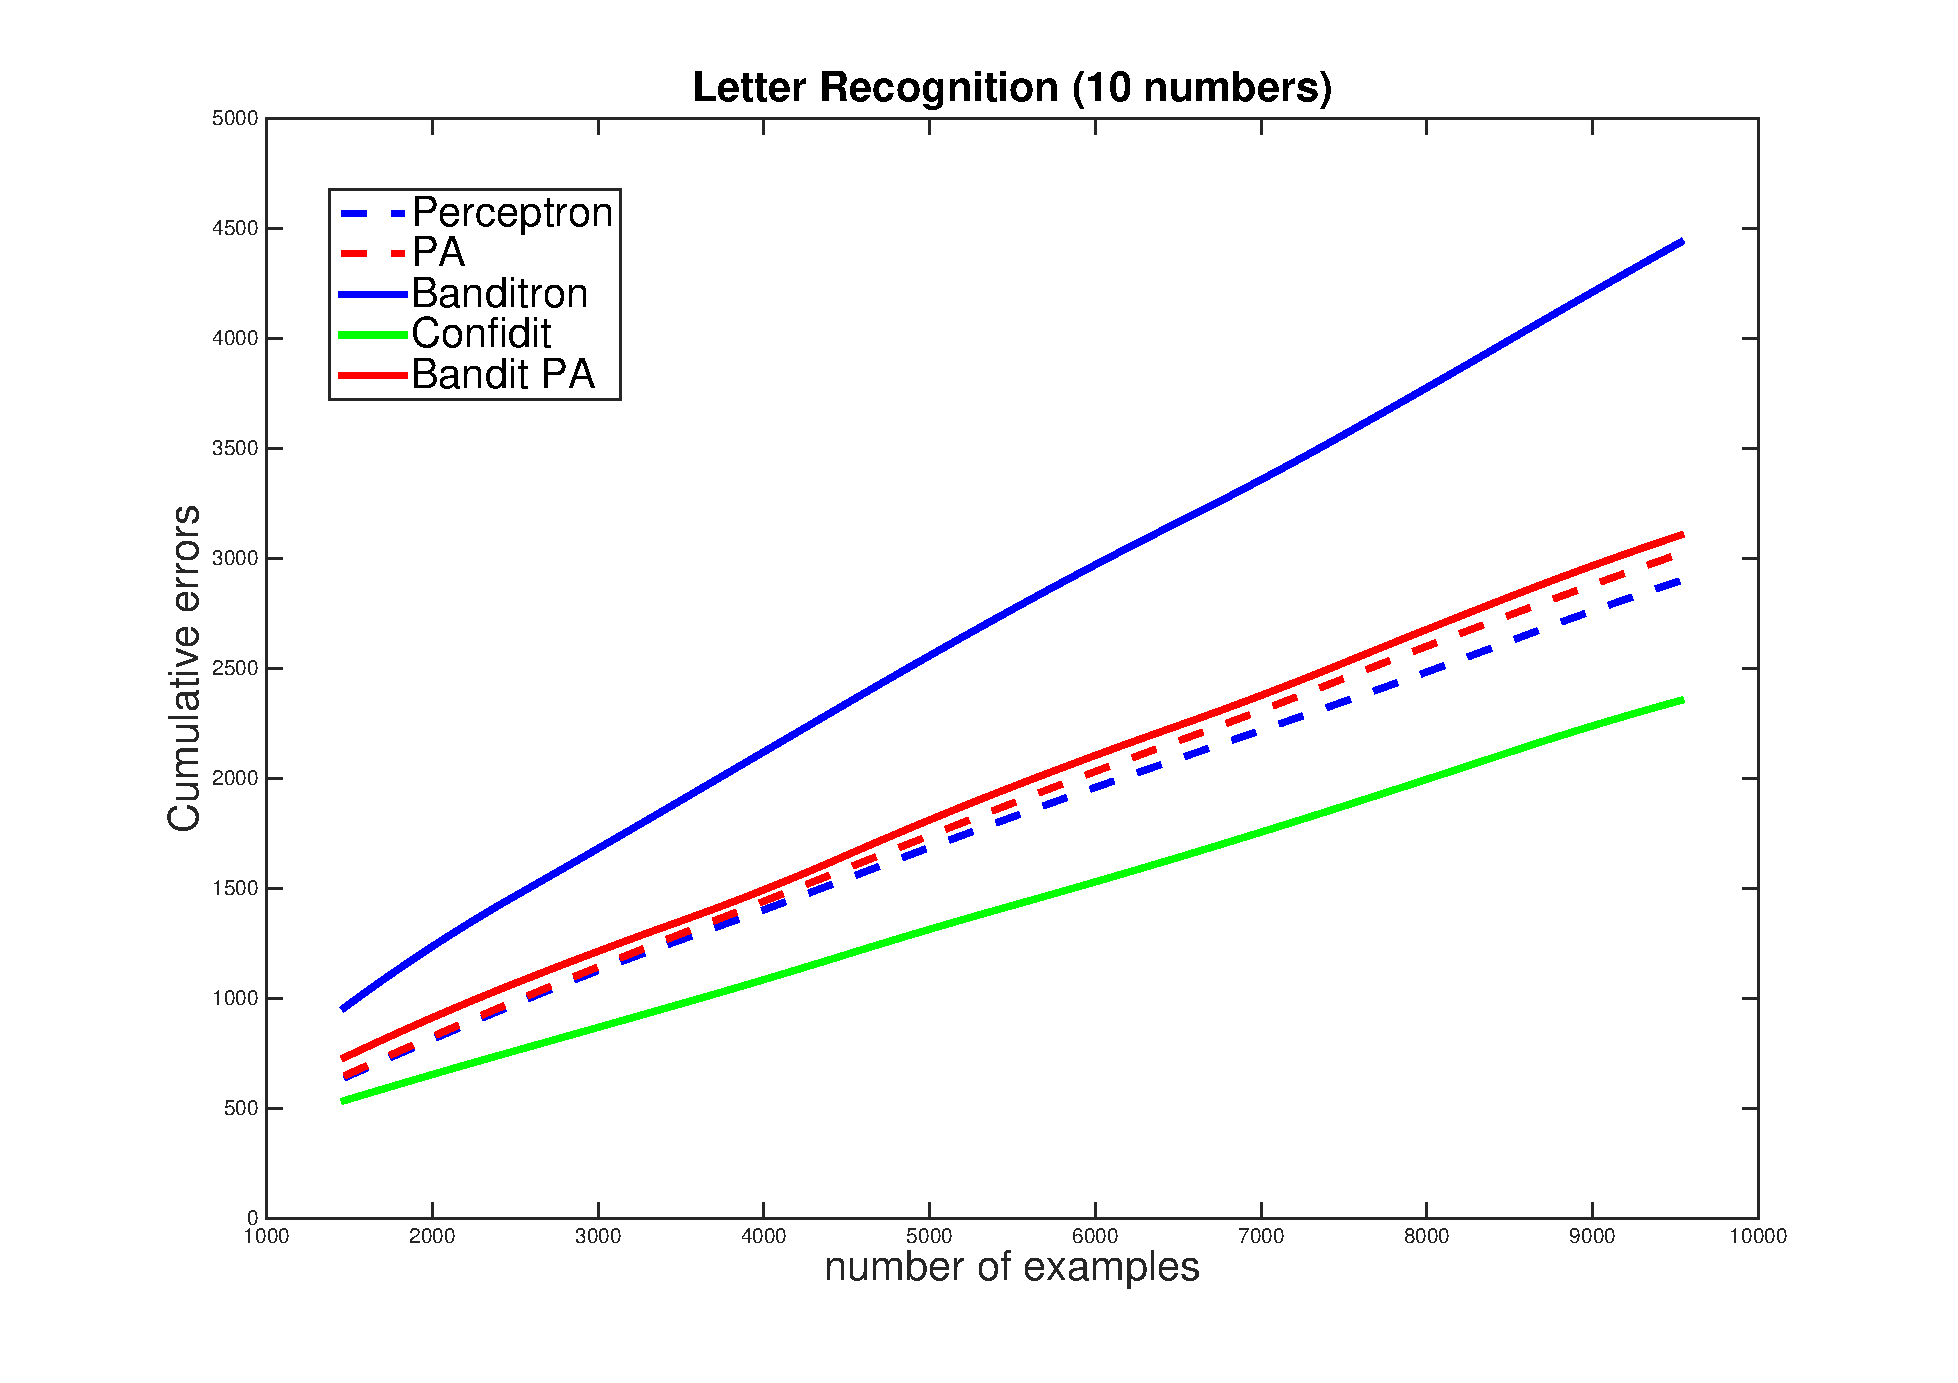
\includegraphics[width=\linewidth]{figs/10LR.eps}}
	\caption{Cumulative Errors on the real data set of Letter Recognition (10 numbers).}
	\label{pic:BPALR10}
\end{figure}

\begin{figure}[h!]
	\centerline{
		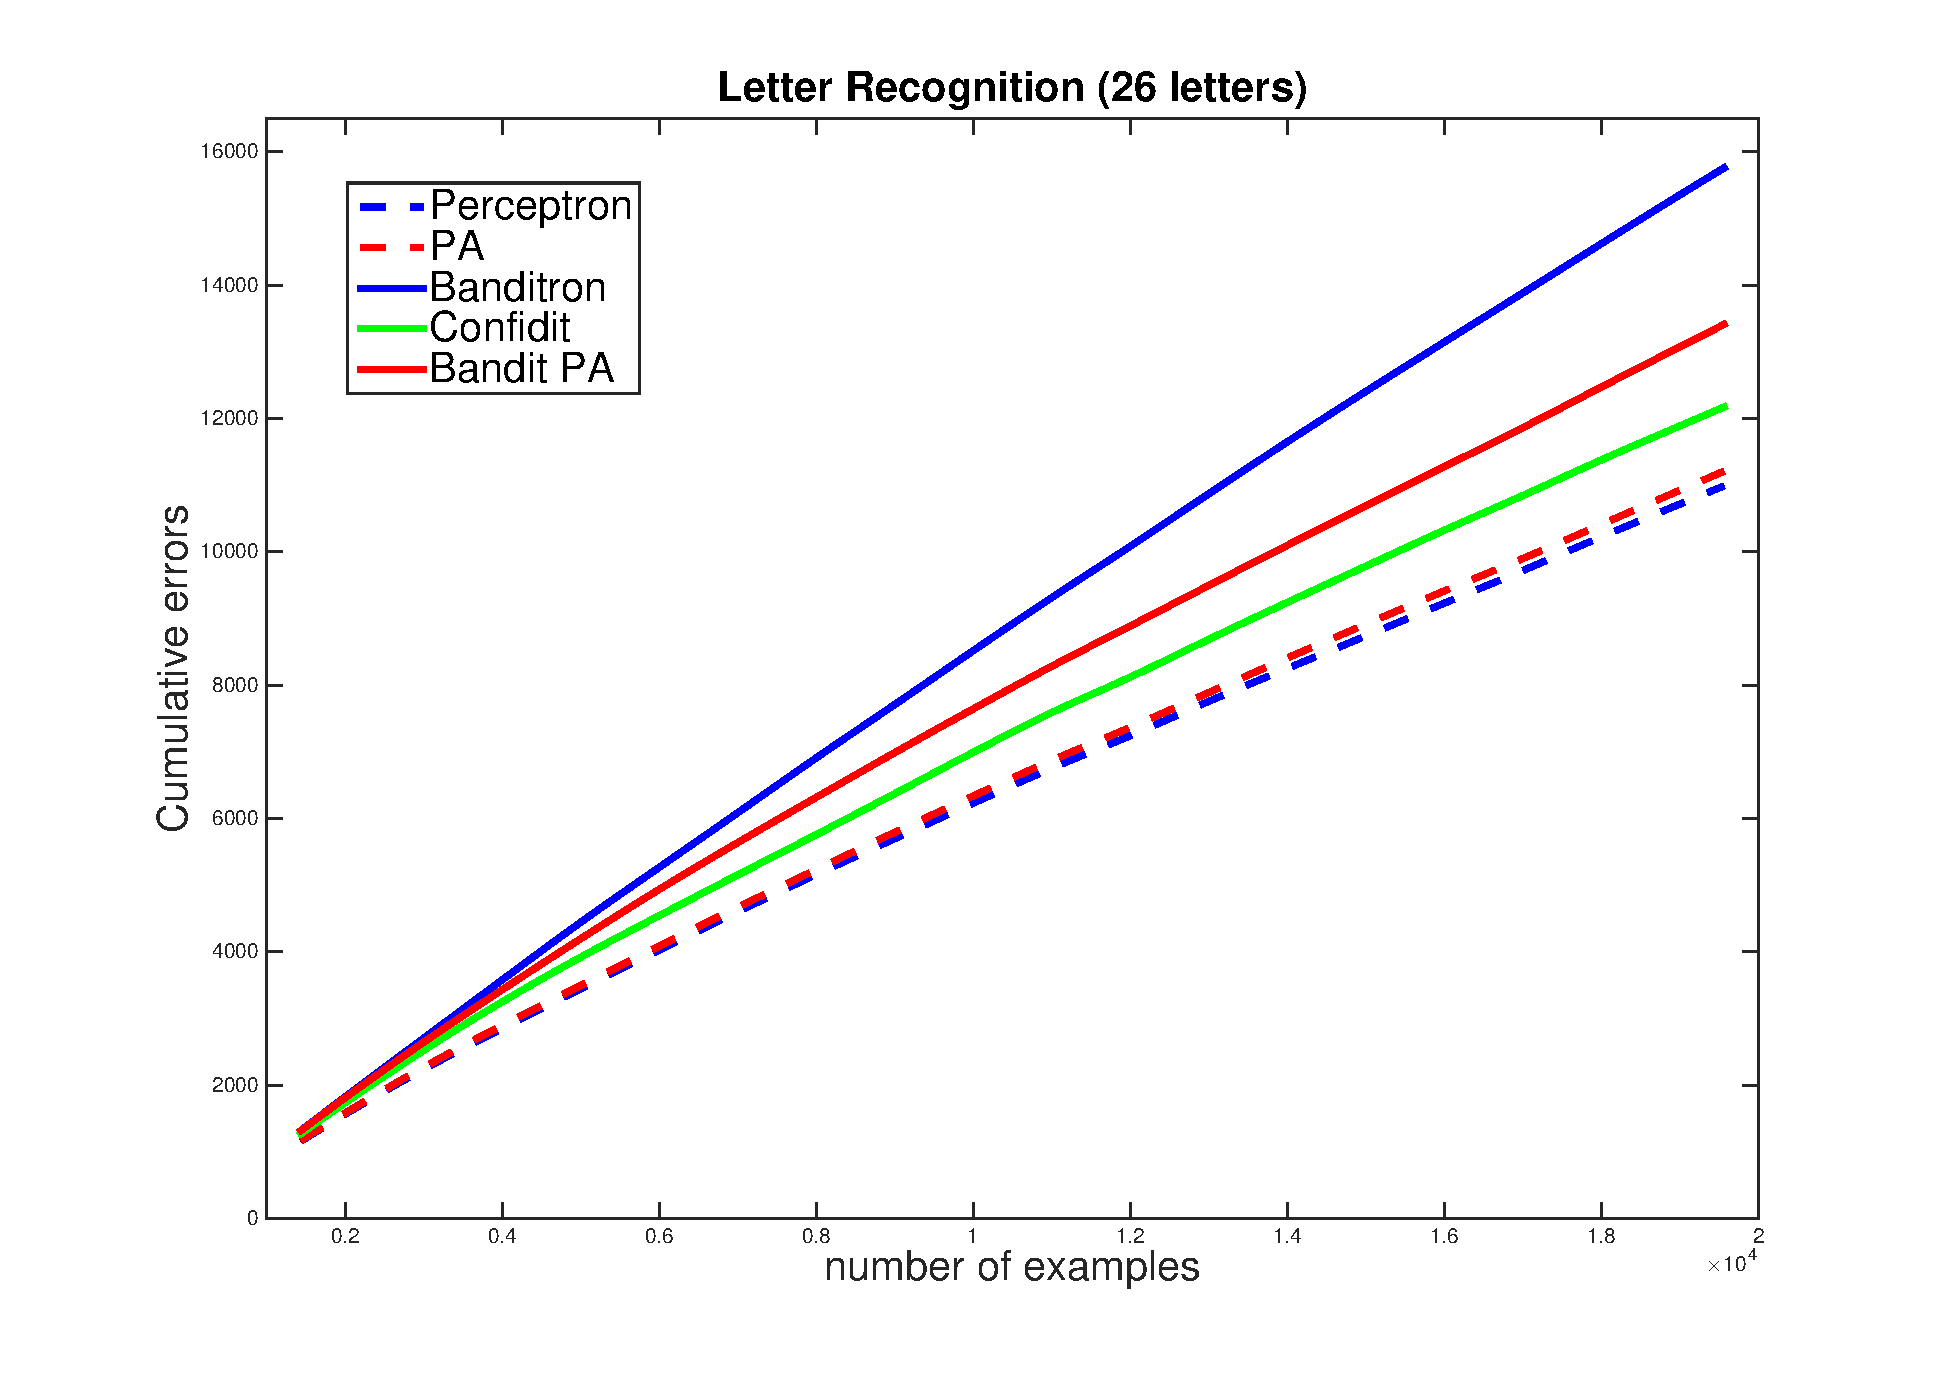
\includegraphics[width=\linewidth]{figs/26LR.eps}}
	\caption{Cumulative Errors  on the real data set of Letter Recognition (26 Letters).}
	\label{pic:BPALR26}
\end{figure}

\begin{figure}[h!]
	\centerline{
		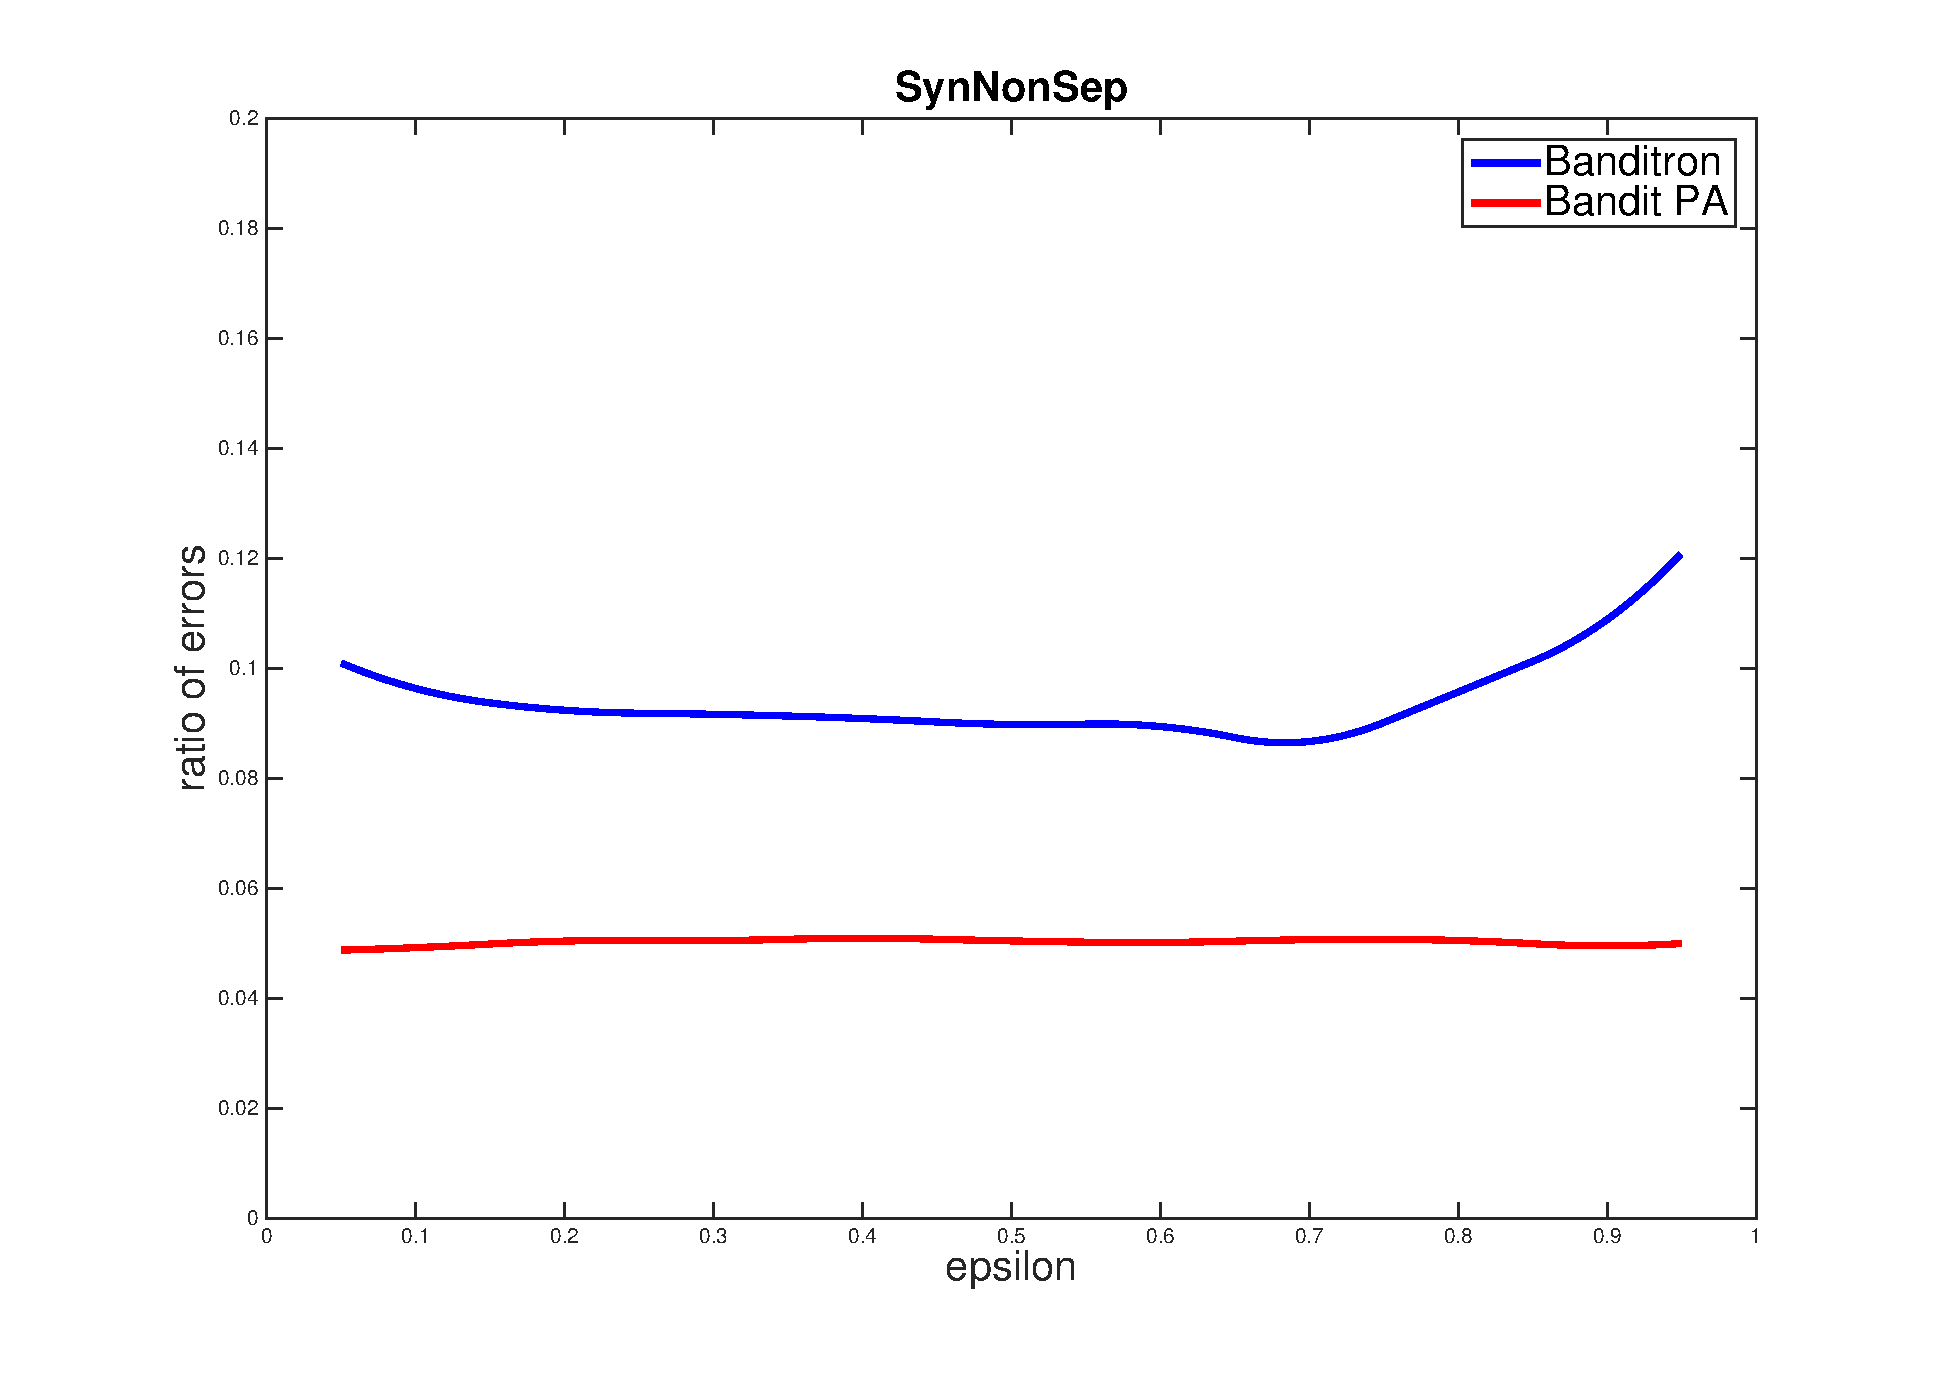
\includegraphics[width=\linewidth]{figs/SynNonSep_gamma.eps}}
	\caption{Average error of Banditron and BPA for parameter's value $\epsilon$ on the data set of SynNonSep. }
	\label{pic:BPASNSerr}
\end{figure}

\begin{figure}[h!]
	\centerline{
		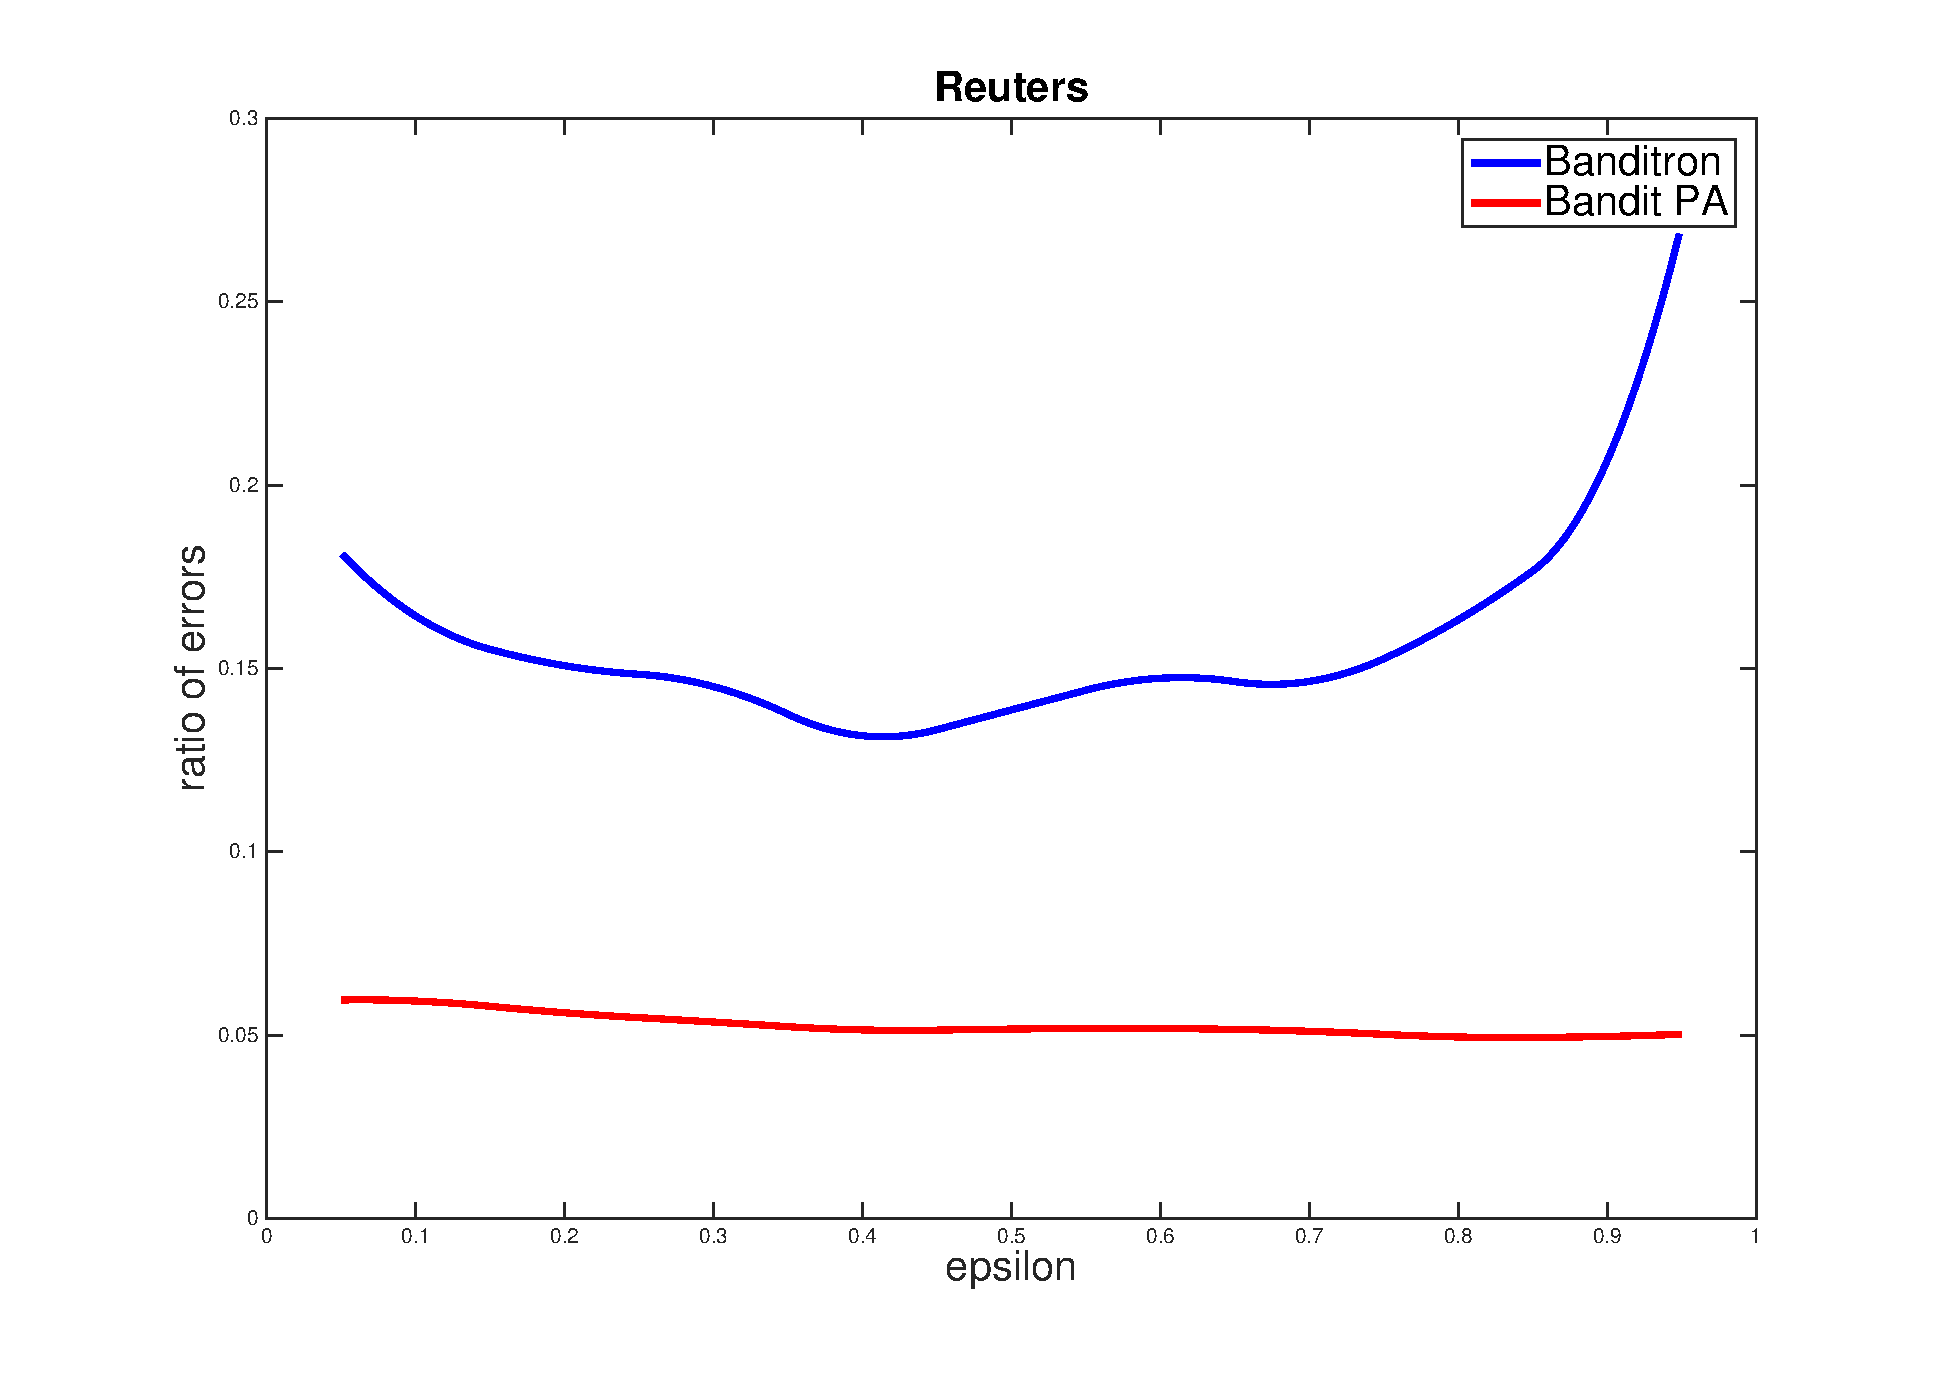
\includegraphics[width=\linewidth]{figs/Reuters_gamma.eps}}
	\caption{Average error of Banditron and BPA for parameter's value $\epsilon$ on the data set of Reuters.}
	\label{pic:BPARCVerr}
\end{figure}

\begin{figure}[h!]
	\centerline{
		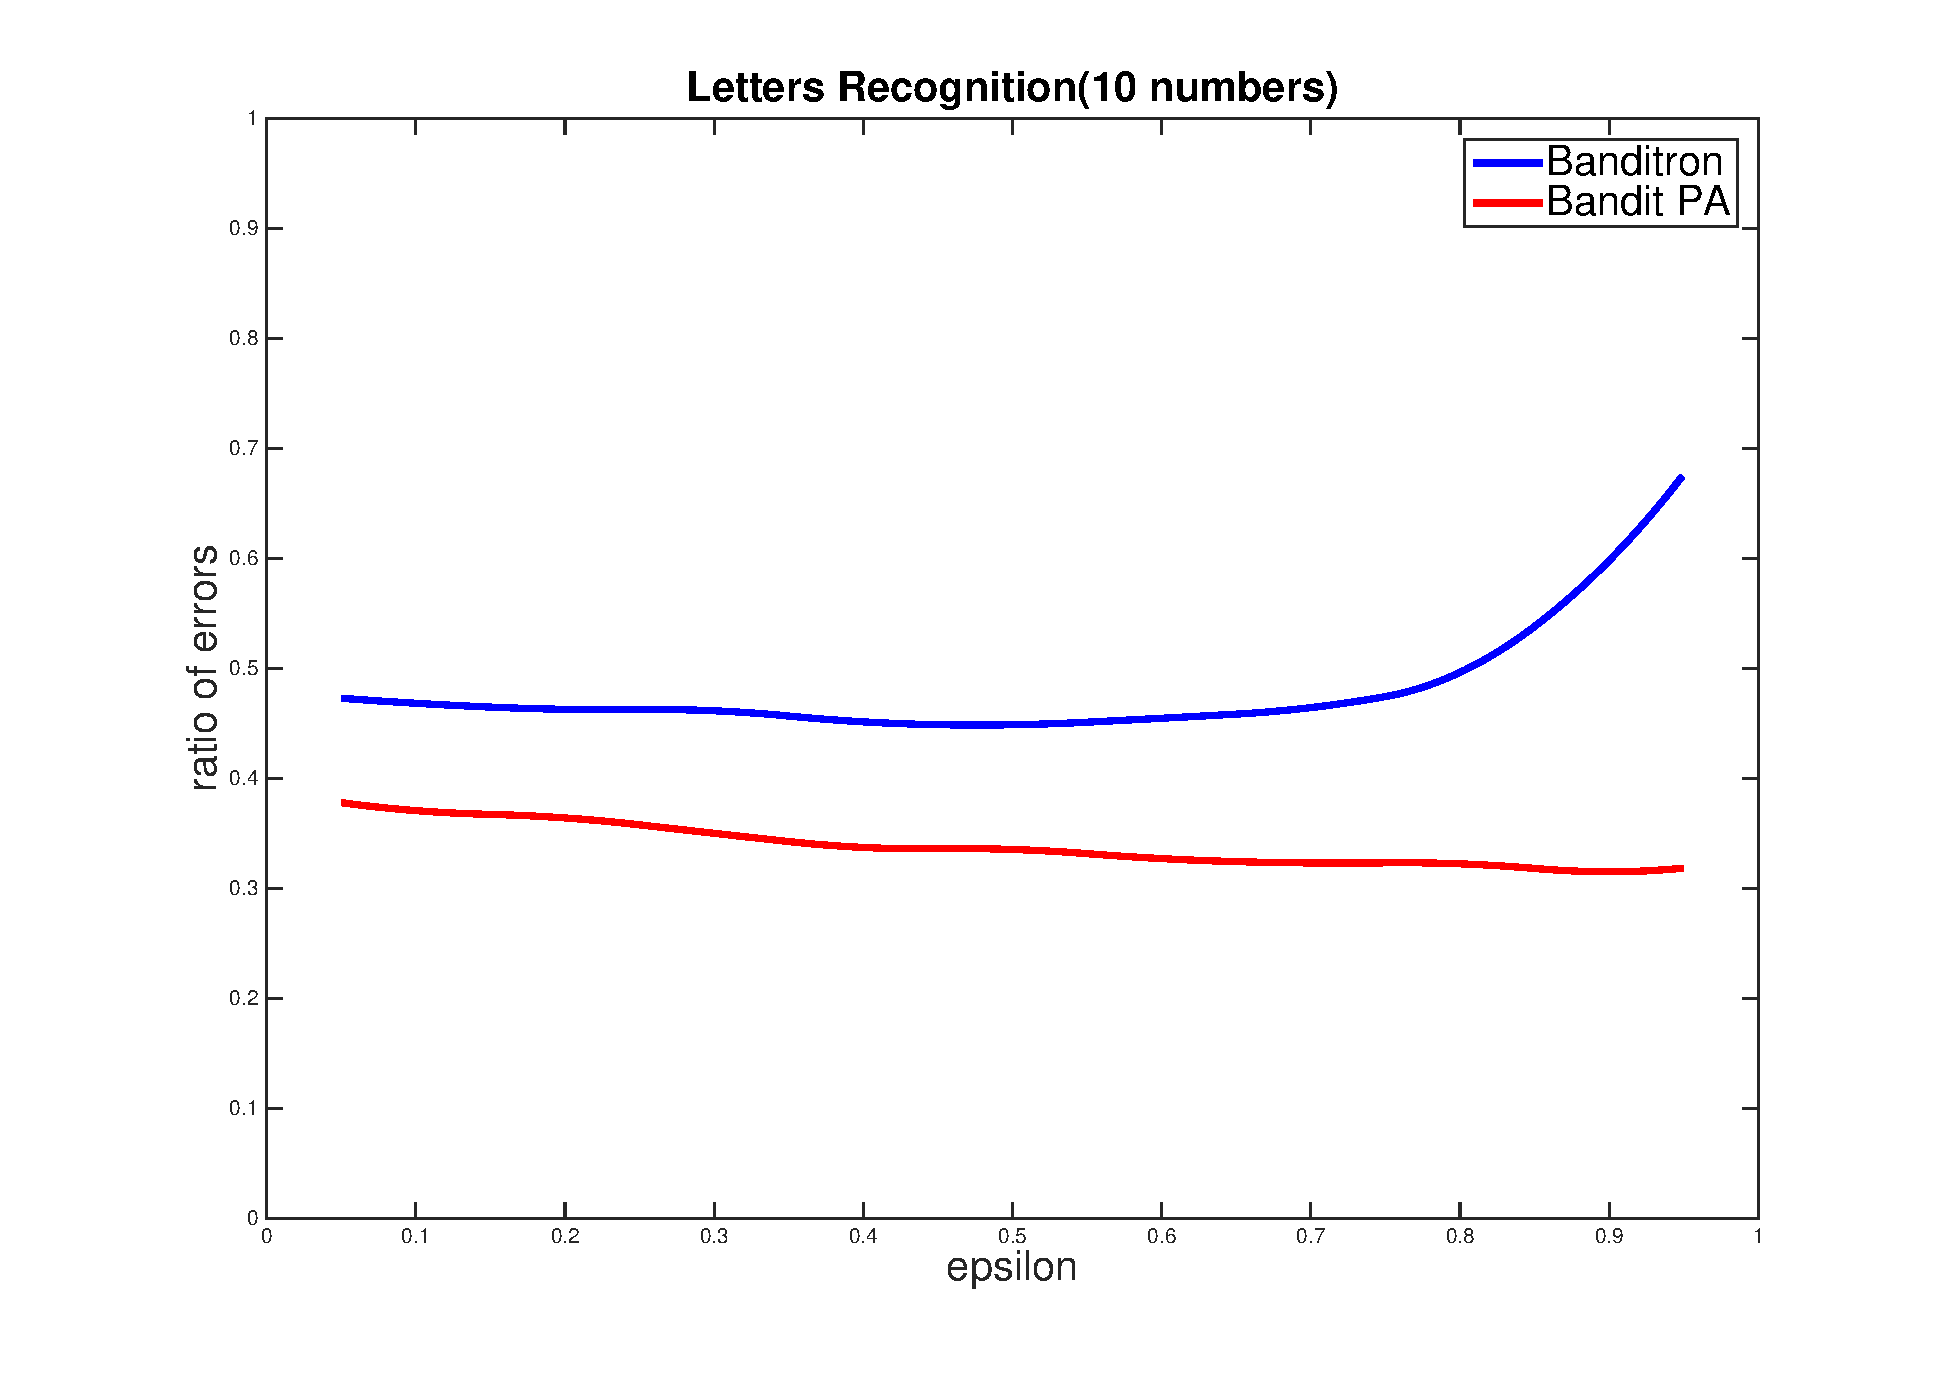
\includegraphics[width=\linewidth]{figs/10LR_gamma.eps}}
	\caption{Average error of Banditron and BPA for parameter's value $\epsilon$ on the data set of Letter Recognition.}
	\label{pic:BPALRerr}
\end{figure}


\subsection{Non-linearly separable datasets}

In this section, we take two datasets to evaluate and analyze the effect of these algorithm in Reproducing Kernel Hilbert Space.

\vspace{1.5ex}
\textbf{Data description}
The first dataset denoted by Pendigits, is a real data and created by E.Alpaydin and Fevzi.Alimoglu \cite{alimoglu1996combining,Alimoglu96methodsof}. 
It  collected 250samples from 44 writers. All writers are asked to write 250 digits in random order inside boxes of 500 by 500 tablet pixel resolution. 
Here, the dataset is part of original one. It contains 7494 instances, 16 features and 10 classes. 

The second dataset denoted by `Segment'\cite{Lichman:2013}. This dataset contains 2310 instances, all of them were drawn randomly from a database of 7 outdoor images. The images were handsegmented to create a clasification for every pixel. Each instance is a $3\times 3$ region. It's a real dataset, with 19 features and 7 classes. More details could be referred to the data site ``UCI''.

\vspace{1.5ex}
%\textcolor{red}{OK-- Il faut donner la formule des noyaux lineaire et Laplace}
\textbf{Algorithm}
Here, we take algorithms Banditron (in RKHS), KBPA and KSGD to compare. In order to perform the effect of RKHS, we choose KBPA in linear model as the reference object and choose \textbf{Laplace} for the kernel function. Its form looks like the following formulate.
\[K_{Laplace}(x,y) = \exp{\left(-\frac{\parallel{x-y}\parallel}{\sigma}\right)}\]
So, all participant algorithms contains: KBanditron, KBPA (linear), KBPA (Laplace), and KSGD (Laplace). For each dataset, the parameter of kernel function is different. By cross-validation way, we choose $\eta = 1$ of model `Laplace' for dataset Pendigits and $\eta = 10$ for dataset `Segment'. For KSGD, the truncated number is 500 for dataset Pendigits, and 200 for Segment.

\vspace{1.5ex}
\textbf{Result}
We mainly analyze these experiments from the following aspects. 

Average training time for each instance:  we observe the training time of every instance $\{t_1,t_2,\dots,t_n\}$; then divide 100 ordering examples into one group $g_1 = \{t_1,\dots,t_{100}\}$,
$\dots$, $g_i = \{t_{1+100*(i-1)},\dots, t_{100*i}\}$; finally, the average training time for instances of group $g_i$ can be calculated by $\overline{t_i} = \frac{1}{100}\sum_{s=1+100*(i-1)}^{100*i} t_s$. 

Average error rate: $e_i = \sum_{s=1+100*(i-1)}^{100\times i}\mathbf{1}_{\hat{y}_t = y_t}/100$ this measure is calculated by the same way.

Cumulative Errors: calculate the total number of past errors.

In Figure~\ref{pic:PKT}, it gives the result of average training time on based dataset ``Pendigits''.  From this result, the training time of three kernel algorithms increases linearly along with the number of training instances. Only the linear model is stable. From the theoretical perspective, Banditron always adds a new example passively for its support vector. Algorithm KSGD only adds a new example for its support vector if its classifier makes a bad prediction, otherwise the number of support vector is limited by the truncated parameter. Algorithm KBPA adds a new example for its support vector if and only if its predicted loss not equals to zero. So its number of support vector will increase all the time until it can make good prediction with no loss.

In Figure~\ref{pic:PKM} and Figure~\ref{pic:PKCM}, accumulative errors of algorithm KBPA firstly tend to a stable, others still increase linearly. That is because KBPA accumulates all good support vectors, KSGD only accumulates several recent support vectors and Kernel Banditron always accumulates new instance as negative support vector.

In Figure~\ref{pic:SKT}, it is about the average training time on dataset ``Segment''.  The training time of Kernel Banditron still increases linearly, while the training time of KSGD and KBPA are as stable as linear model after a small period of increasing linearly. KSGD reaches the limited number of support vector, and KBPA quickly gets enough support vectors to make a good prediction. It could show that this dataset is separable. 

In Figure~\ref{pic:SKM} and Figure~\ref{pic:SKCM}, we can observe that KBPA and KSGD performed obviously better than the other two.  Two kernel algorithms have ability to solve non-linear classification with Bandit Feedback. Considering the scale of classifier, we can use more efficient algorithm KBPA if dataset is separable, otherwise we use KSGD.

\begin{figure}[h!]
	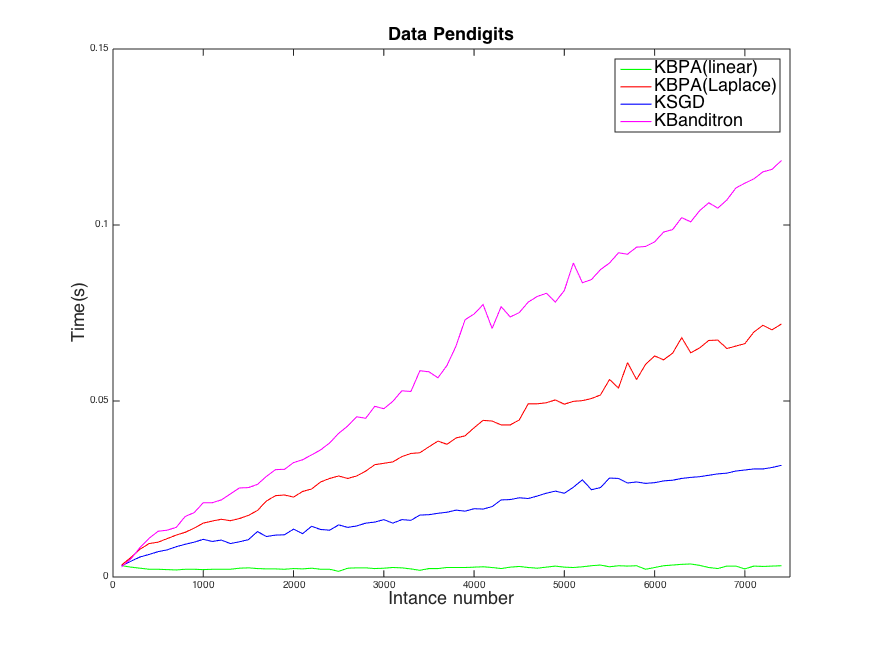
\includegraphics[width=\linewidth]{figs/Pendigits_kernel_T.png}
	\caption{Average training time for each instance of Data Pendigits.}
	\label{pic:PKT}
\end{figure}

\begin{figure}[h!]
	\centerline{
		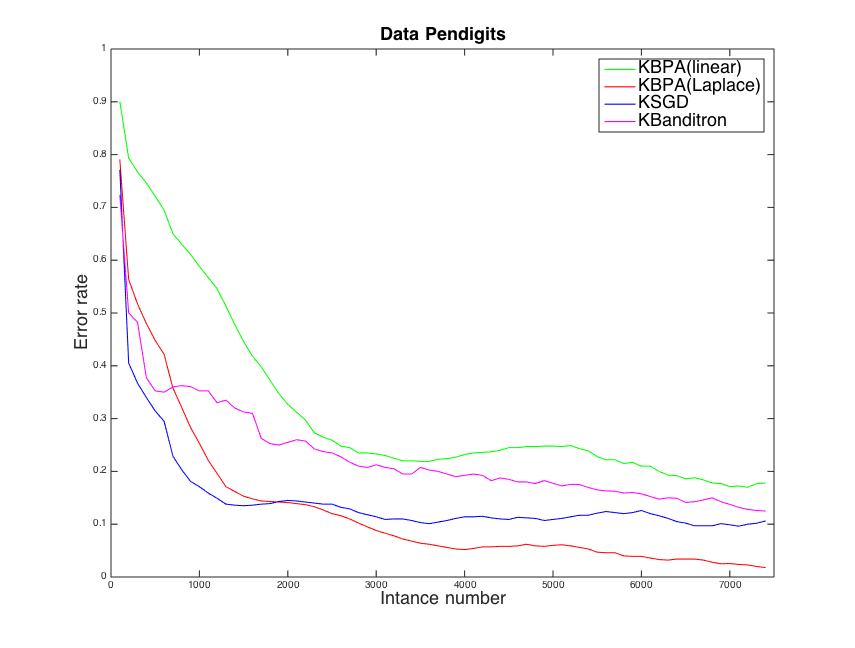
\includegraphics[width=\linewidth]{figs/Pendigits_kernel_M.png}}
	\caption{Average error rate for each instance of Data Pendigits}
	\label{pic:PKM}
\end{figure}

\begin{figure}[h!]
	\centerline{
		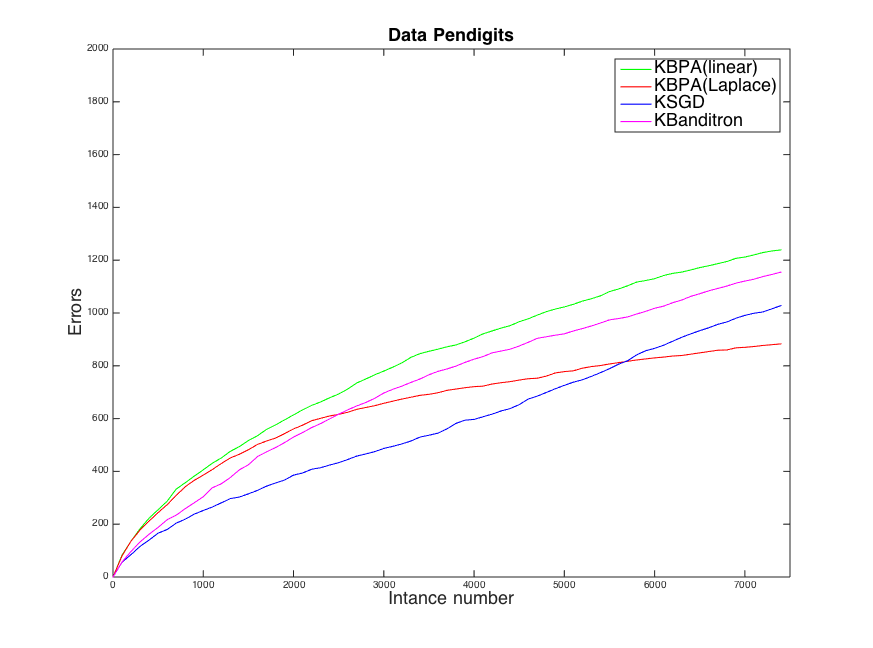
\includegraphics[width=\linewidth]{figs/Pendigits_kernel_CM.png}}
	\caption{Cumulative Errors of Data Pendigits}
	\label{pic:PKCM}
\end{figure}

%\begin{figure}[h!]
%\label{pic:PKR}
%\centerline{
%\includegraphics[scale = 0.4]{fig05/mc/Pendigits_kernel_R.png}}
%\caption{Cumulative loss of Data Pendigits}
%\end{figure}

\begin{figure}[h!]
	\centerline{
		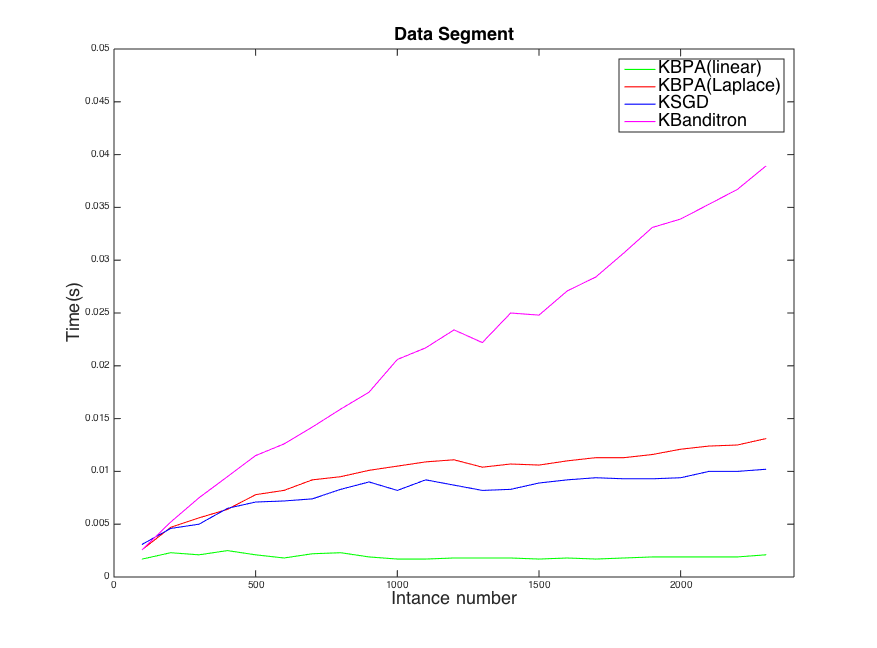
\includegraphics[width=\linewidth]{figs/Segment_kernel_T.png}}
	\caption{Average training time for each instance of Data Segment.}
	\label{pic:SKT}
\end{figure}

\begin{figure}[h!]
	\centerline{
		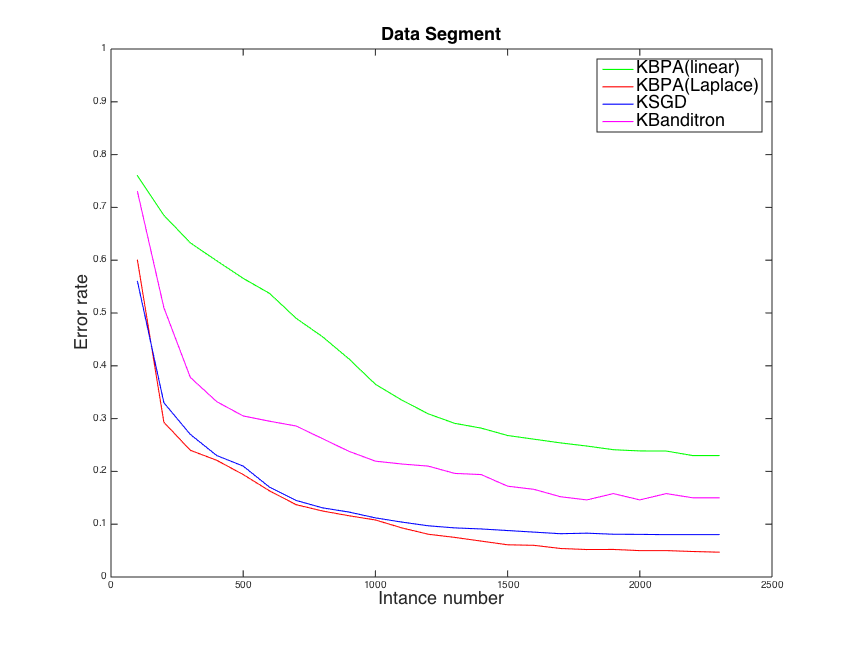
\includegraphics[width=\linewidth]{figs/Segment_kernel_M.png}}
	\caption{Average error rate for each instance of Data Segment}
	\label{pic:SKM}
\end{figure}

\begin{figure}[h!]
	\centerline{
		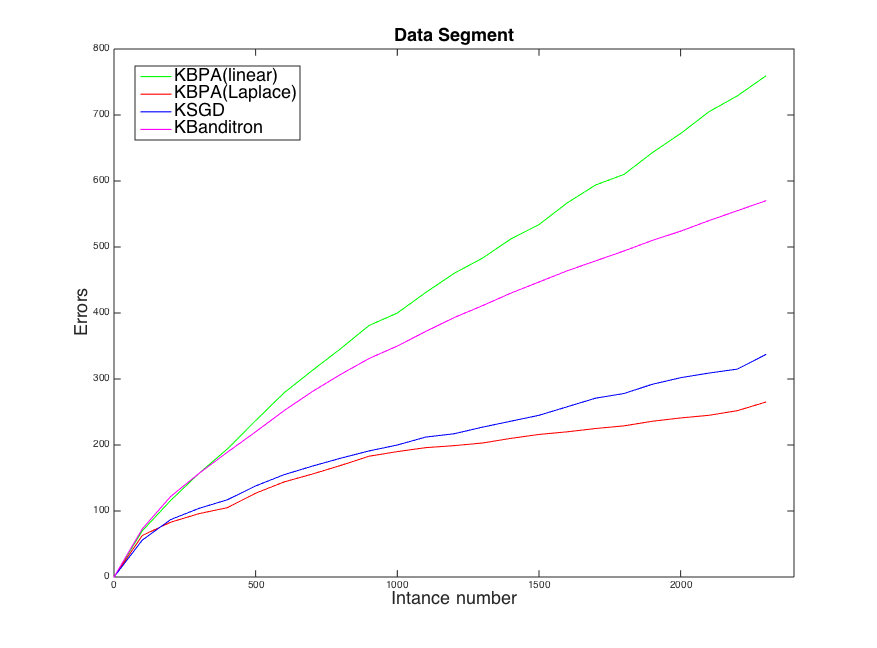
\includegraphics[width=\linewidth]{figs/Segment_kernel_CM.png}}
	\caption{Cumulative Errors of Data Segment}
	\label{pic:SKCM}
\end{figure}

%\begin{figure}[h!]
%\label{pic:SKR}
%\centerline{
%\includegraphics[scale = 0.4]{fig05/mc/Segment_kernel_R.png}}
%\caption{Cumulative loss of Data Segment}
%\end{figure}
%\subsection{Conclusion}
\section{Conclusion}
\label{sec:conclusion}
{Conclusion}
\label{subsec:BPAC}

We proposed a novel algorithm for online multiclass classification with bandit feedback. By the advantage of PA max-margin principle, BPA appears effective to address the bandit online learning setting. Its main advantage is its linear complexity in space that allows to deal with high dimensional data sets and a large number of classes, on the contrary to second-order methods. The practicability of this algorithm is verified theoretically by showing a competitive loss bound.

Moreover, experimental evaluation shows that BPA performs better than other algorithms on  real datasets, even better than the algorithms with full feedback on the data sets non-separable.


la conclusion est qu’une information minimale (binaire) offre des capacites de convergence comparable en ordre de grandeur à une information complète.


\bibliography{cap2016}

\end{document}

%%% Local Variables: 
%%% mode: latex
%%% TeX-master: t
%%% End: 
